%% ut-thesis.tex -- document template for graduate theses at UofT
%%
%% Copyright (c) 1998-2013 Francois Pitt <fpitt@cs.utoronto.ca>
%% last updated at 16:20 (EDT) on Wed 25 Sep 2013
%%
%% This work may be distributed and/or modified under the conditions of
%% the LaTeX Project Public License, either version 1.3c of this license
%% or (at your option) any later version.
%% The latest version of this license is in
%%     http://www.latex-project.org/lppl.txt
%% and version 1.3c or later is part of all distributions of LaTeX
%% version 2005/12/01 or later.
%%
%% This work has the LPPL maintenance status "maintained".
%%
%% The Current Maintainer of this work is
%% Francois Pitt <fpitt@cs.utoronto.ca>.
%%
%% This work consists of the files listed in the accompanying README.

%% SUMMARY OF FEATURES:
%%
%% All environments, commands, and options provided by the `ut-thesis'
%% class will be described below, at the point where they should appear
%% in the document.  See the file `ut-thesis.cls' for more details.
%%
%% To explicitly set the pagestyle of any blank page inserted with
%% \cleardoublepage, use one of \clearemptydoublepage,
%% \clearplaindoublepage, \clearthesisdoublepage, or
%% \clearstandarddoublepage (to use the style currently in effect).
%%
%% For single-spaced quotes or quotations, use the `longquote' and
%% `longquotation' environments.


%%%%%%%%%%%%         PREAMBLE         %%%%%%%%%%%%

%%  - Default settings format a final copy (single-sided, normal
%%    margins, one-and-a-half-spaced with single-spaced notes).
%%  - For a rough copy (double-sided, normal margins, double-spaced,
%%    with the word "DRAFT" printed at each corner of every page), use
%%    the `draft' option.
%%  - The default global line spacing can be changed with one of the
%%    options `singlespaced', `onehalfspaced', or `doublespaced'.
%%  - Footnotes and marginal notes are all single-spaced by default, but
%%    can be made to have the same spacing as the rest of the document
%%    by using the option `standardspacednotes'.
%%  - The size of the margins can be changed with one of the options:
%%     . `narrowmargins' (1 1/4" left, 3/4" others),
%%     . `normalmargins' (1 1/4" left, 1" others),
%%     . `widemargins' (1 1/4" all),
%%     . `extrawidemargins' (1 1/2" all).
%%  - The pagestyle of "cleared" pages (empty pages inserted in
%%    two-sided documents to put the next page on the right-hand side)
%%    can be set with one of the options `cleardoublepagestyleempty',
%%    `cleardoublepagestyleplain', or `cleardoublepagestylestandard'.
%%  - Any other standard option for the `report' document class can be
%%    used to override the default or draft settings (such as `10pt',
%%    `11pt', `12pt'), and standard LaTeX packages can be used to
%%    further customize the layout and/or formatting of the document.

%% *** Add any desired options. ***
%\documentclass[twoside]{ut-thesis}


%%\newcommand{\myDocOptions}{10pt,twoside,openany,singlespaced,normalmargins,draft}

%% debug
%\newcommand{\myDocOptions}{11pt,a4,twoside,openany,singlespaced,normalmargins}
%\newcommand{\myDocOptions}{11pt,a4paper,oneside,openright,onehalfspaced,normalmargins}

%% production
\newcommand{\myDocOptions}{11pt,twoside,openright,onehalfspaced,normalmargins}


%\newcommand{\myDocOptions}{12pt,twoside,openany,oneandahalfspaced,normalmargins}
%\newcommand{\myDocOptions}{12pt,twoside,openany,doublespaced,normalmargins} %% ,draft}


\documentclass[\myDocOptions]{ut-thesis}




%% *** Add \usepackage declarations here. ***
%% The standard packages `geometry' and `setspace' are already loaded by
%% `ut-thesis' -- see their documentation for details of the features
%% they provide.  In particular, you may use the \geometry command here
%% to adjust the margins if none of the ut-thesis options are suitable
%% (see the `geometry' package for details).  You may also use the
%% \setstretch command to set the line spacing to a value other than
%% single, one-and-a-half, or double spaced (see the `setspace' package
%% for details).

\usepackage{url,alltt}
\usepackage{paralist, xspace}
\usepackage{caption}
\usepackage{subcaption}
\usepackage{graphicx}
\usepackage{wrapfig}
\usepackage{times}
\usepackage{amssymb,amsmath,pifont,footnote}
\usepackage{latexsym,pdfpages}
\usepackage{array,verbatim}
\usepackage{stmaryrd,ifsym}
\usepackage{algorithmic,algorithm}
\usepackage{gastex} % compile twice when pictures have changed.
\usepackage{parcolumns}
\usepackage{listings}
\usepackage{color}
\usepackage{hyperref}
\usepackage{cleveref}
\usepackage{enumitem}
\usepackage{amsthm}
\usepackage{pdfpages}
\usepackage{algorithmic}
%%%%%%%%%%%%%%%%%%%%%%%%%%%%%%%%%%%%%%%%%%%%%%%%%%%%%%%%%%%%%%%%%%%%%%%%
%%                                                                    %%
%%                   ***   I M P O R T A N T   ***                    %%
%%                                                                    %%
%%  Fill in the following fields with the required information:       %%
%%   - \degree{...}       name of the degree obtained                 %%
%%   - \department{...}   name of the graduate department             %%
%%   - \gradyear{...}     year of graduation                          %%
%%   - \author{...}       name of the author                          %%
%%   - \title{...}        title of the thesis                         %%
%%%%%%%%%%%%%%%%%%%%%%%%%%%%%%%%%%%%%%%%%%%%%%%%%%%%%%%%%%%%%%%%%%%%%%%%

%% *** Change this example to appropriate values. ***
\degree{Master of Science}
\department{Computer Science}
\gradyear{2016}
\author{Orr Fischer}
\title{Topics in Distributed Computing and Simultaneous Multi-Party Communication Complexity}

%% *** NOTE ***
%% Put here all other formatting commands that belong in the preamble.
%% In particular, you should put all of your \newcommand's,
%% \newenvironment's, \newtheorem's, etc. (in other words, all the
%% global definitions that you will need throughout your thesis) in a
%% separate file and use "\input{filename}" to input it here.

\sloppy
%\pagestyle{empty}

\definecolor{dkgreen}{rgb}{0,0.6,0}
\definecolor{gray}{rgb}{0.5,0.5,0.5}
\definecolor{mauve}{rgb}{0.58,0,0.82}

\lstset{%frame=tb,
%  language=Java,
  %aboveskip=3mm,
  %belowskip=3mm,
  %showstringspaces=false,
  %columns=flexible,
  basicstyle={\small\ttfamily},
  %numbers=none,
%  basicstyle=\tiny,
%  numberstyle=\tiny\color{gray},
%  keywordstyle=\color{blue},
%  commentstyle=\color{dkgreen},
%  stringstyle=\color{mauve},
  %breaklines=true,
  %breakatwhitespace=true
%  tabsize=3
}
\setlist{nolistsep}



%\newtheorem{thm}{Theorem} %Added
%\newtheorem{notat}[thm]{Notations}
%%\newtheorem{lem}[thm]{Lemma}
%\newtheorem{lem}{Lemma}
%\newtheorem{WorkAround}{Lemma}
%%\newtheorem{prop}[thm]{Proposition}
%\newtheorem{prop}{Proposition}
%%\newtheorem{rem}[thm]{Remark}
%\newtheorem{rem}{Remark}
%\newtheorem{prob}{Problem}
%\newtheorem{fact}{Fact}
%
%%\newtheorem{cor}[thm]{Corollary}
%\newtheorem{cor}{Corollary}
%\newtheorem{Obs}{Observation}
%%\newenvironment{prop}{\theoremlike{Proposition}}{\par\medskip}
%%\theoremlike{prop}{<caption>}[<within>]
%%{\bfseries}{\itshape}
%%\newtheorem{defn}[thm]{Definition}
%\newtheorem{defn}{Definition}
%\newtheorem{examp}{Example}
%\newtheorem{example}{Example}
%%
%\newtheorem{dfn}[thm]{Definition}

%\newcommand{\pfbox}{\quad\hspace*{\fill}$\Box$}
%\newcommand{\pfbox}{\qed}

%\newenvironment{proof}{\noindent {\bf Proof}~}{\pfbox\bigskip}
% \renewcommand{\baselinestretch}{0.95}
%\renewcommand{\baselinestretch}{0.975}

% \setlength{\bibsep}{0.40ex}

\newcommand{\Nat}{\ensuremath{\mathbb{N}}}
\newcommand{\Rea}{\ensuremath{\mathbb{R}}}
\newcommand {\exptime} {\textsc{exptime}}
\def\Unbound{\mathit{Unbound}}
\def\Dense{\mathit{Dense}}
\def\blim{\mathit{base}-\lim}
\def\class{\mathcal{ C}}
\def\fF{\mathfrak{F}}
\def\clos{\mathit{Cl}}
\def\shuf{\mathit{shuffle}}
\def\fset{finite-set }
%\newcommand{\}{\mathit{Hin}}
\newcommand{\hin}{\mathit{Hin}}
\newcommand{\Flag}{\mbox{Updated}}
\newcommand{\false}{\mbox{False}}
\newcommand{\true}{\mbox{True}}
\newcommand{\TL}{\mathit{TL}}

\def\vp{\varphi}
\def\mG{\mathcal{G}}
\def\rar{\rightarrow}
\def\power{\mathcal{P}}
\def\s{\subseteq}
\def\All{\forall}
\def\we{\wedge}
\def\dep{\mathit{qd}}
\newcommand{\MLO}{\mbox{MLO}}
\newcommand{\FOMLO}{\mbox{FOMLO}}
\def\mL{\mathcal{L}}
\def\mM{\mathcal{M}}
\def\mR{\mathcal{R}}
\def\mI{\mathcal{I}}
\def\mJ{\mathcal{J}}
\def\mN{\mathcal{N}}
\def\MTh{\mathit{MTh}}
\def\HF{\mathit{type}}
\def\Th{\mathit{Th}}
\def\mD{\mathcal{D}}
\def\Form{\mathfrak{Form}}
\def\fS{\mathfrak{S}}
\def\fH{\mathfrak{H}}
\def\nek{\ldots}
\newcommand{\qd}[1]{\mathop{\rm qd}(#1)}
\def\strucmult{\otimes}
\def\typemult{\otimes}
\def\la{\lambda}
\def\close{\mathit{Closed}}
\def\win{\mathit{Win}}
\def\Realize{\mbox{Realize}}
\def\Dsynth{\mbox{Dsynth}}
\def\Fsynth{\mbox{Fsynth}}

\def\st{\mathit{st}}
\def\type{\mathit{type}}
\def\ttype{\mathit{ptype}}
\def\sgame{\mathit{Game}}
\def\res{\mathit{res}}
\def\win{\mathit{win}}
\def\Win{\mathit{Win}}
\def\Dwin{\mathit{Dwin}}
\def\Fswin{\mathit{Fswin}}
\def\Mult{\mathit{Mult}}
\newcommand{\G}[2]{R(#1,#2)}
\def\owin{\mbox{Or-win}}
\def\scaus{\mbox{I-Player-strategy}}
\def\caus{\mbox{II-Player-strategy}}
\def\upd{\mbox{next}}
\def\upl{\Delta}
\def\out{\mbox{out}}
\DeclareMathOperator{\rank}{rank}
\DeclareMathOperator{\weight}{weight}
\DeclareMathOperator{\col}{col}
\def\Dl{D^-}
\def\Dr{D^+}
\def\type{\mathit{type}}
\def\rest{\lfloor}
\def\dom{\partial}
\DeclareMathOperator{\Llim}{llim} \DeclareMathOperator{\Rlim}{rlim}
\def\aaut{\mathfrak{ A}}
\def\baut{\mathfrak{ B}}
\def\abasis{B}
\newcommand{\powerset}[1]{\mathcal{P}({#1})}
\newcommand{\arun}{\rho}
\newcommand{\AL}{{\rm always}}
\def\next{\mathit{next}}
\def\word{\mathit{s}}

\def\Left{\mathit{Left}}
\def\Right{\mathit{Right }}
\def\ovarphi{{\overline\varphi}}
\def\Neg{\mathit{Neg}}
\def\Id{\mathit{Id}}
\def\Conj{\mathit{Conj}}
\def\Disj{\mathit{Disj}}
\def\tr{\mathit{Tr}}
\def\diamonds{\overleftarrow{\diamondsuit}}
\newcommand{\LE}{\mbox{\it{Q2MLO}$_\exists$}}
\def\Lreg{\class_{reg}}
\def\lab{\mathit{lab}}
\def\Rreg{\mR_{reg}}

\def\One{\mathit{One}}

\newcommand{\simplies}{\DOTSB\Longrightarrow}

%\newif\iffullproofs
%\newif\ifshortproofs
%\newif\iflong
%\newif\iftacas


%%%% for tacas use:
% \fullproofsfalse
% \shortproofstrue
% \longfalse
% \tacastrue

%%%% for tech report use
% \fullproofsfalse
% \shortproofstrue
% \longfalse
% \tacasfalse


%%\proofstrue
%% short version
%\fullproofsfalse
%\shortproofstrue
%\longfalse
%\tacastrue

% % long version
% \fullproofstrue
% \shortproofsfalse
% \longtrue


\newtheorem{theorem}{Theorem}
\newtheorem{remark}{Remark}
\newtheorem{lemma}[theorem]{Lemma}
\newtheorem{claim}[theorem]{Claim}
\newtheorem{conjecture}[theorem]{Conjecture}
\newtheorem{corollary}[theorem]{Corollary}
\newtheorem{fact}[theorem]{Fact}
\newtheorem{proposition}[theorem]{Proposition}
\newtheorem{problem}[theorem]{Problem}
\newtheorem{observation}[theorem]{Observation}
\newtheorem{definition}[theorem]{Definition}
\newtheorem{requirement}[theorem]{Requirement}
\newtheorem{example}[theorem]{Example}
%\newenvironment{proof}[1][Proof]{\begin{trivlist}
%\item[\hskip \labelsep {\bfseries #1}]}
%{\end{trivlist}
%\qed
%}


\newcommand{\exref}[1]{Example~\ref{examp:#1}}
\newcommand{\chapref}[1]{Chapter~\ref{chap:#1}}
\newcommand{\secref}[1]{Section~\ref{sec:#1}}
\newcommand{\lemref}[1]{Lemma~\ref{lem:#1}}
\newcommand{\remref}[1]{Remark~\ref{rem:#1}}
\newcommand{\figref}[1]{Figure~\ref{Fi:#1}}
\newcommand{\thmref}[1]{Theorem~\ref{thm:#1}}
\newcommand{\gV}[1]{\langle \textit{#1}\rangle}
\newcommand{\bid}{\textbf{id}}
\newcommand{\brcv}{\textbf{input}}
\newcommand{\breceive}{\brcv}
\newcommand{\bfrw}{\textbf{output}}
\newcommand{\bforward}{\bfrw}
\newcommand{\bto}{\textbf{to}}
\newcommand{\bif}{\textbf{if}}
\newcommand{\bthen}{\textbf{then}}
\newcommand{\belse}{\textbf{else}}
\newcommand{\binsert}{\textbf{insert}}
\newcommand{\bremove}{\textbf{remove}}
\newcommand{\babort}{\textbf{abort}}
\newcommand{\bskip}{\textbf{skip}}
\newcommand{\bfor}{\textbf{for}}
\newcommand{\bforall}{\textbf{forall}}
\newcommand{\bin}{\textbf{in}}
\newcommand{\band}{\textbf{and}}
\newcommand{\bor}{\textbf{or}}
\newcommand{\bnot}{\textbf{not}}
\newcommand{\bself}{\textbf{self}}
\newcommand{\btuple}[1]{\overline{#1}}
% Learning Switch
\newcommand{\tconnected}{\texttt{connected}}
\newcommand{\tallPorts}{\texttt{allPorts}}
% Firewall
\newcommand{\ttrusted}{\texttt{trusted}}
% Proxy
\newcommand{\tcache}{\texttt{cache}}
\newcommand{\tresponse}{\texttt{response}}
\newcommand{\trequested}{\texttt{requested}}
% Isolation
\newcommand{\tforbidden}{\texttt{forbidden}}
\newcommand{\authorComment}[2]{\textbf{#1:}{\textit{#2}}}
\newcommand{\MVer}{\texttt{MuteVeri}}
\newcommand{\N}{\mathbb{N}}
\newcommand{\authorNote}{}
% Round-Robin
\newcommand{\tnextport}{\texttt{nextport}}

\newcommand{\bdo}{\textbf{do}}
\newcommand{\bwhile}{\textbf{while}}
\newcommand{\bforeach}{\textbf{foreach}}
\newcommand{\breturn}{\textbf{return}}
\newcommand\scalemath[2]{\scalebox{#1}{\mbox{\ensuremath{\displaystyle #2}}}}



%%%% Macros from main

\newcommand{\TODO}[1]{{\color{red} \textit{ \textbf{ TODO: #1 }}}}


\newcommand{\tuple}[1]{\left(#1\right)}
\newcommand{\bliml}{\mathit{Base}_{\underrightarrow{\lim }} }
\newcommand{\blimr}{\mathit{Base}_{\underleftarrow{\lim }} }
\def\set#1{\{ #1 \}}
\def\th{\lambda}

\newcommand{\SC}{\mathcal{SFOT_{\cA}}}
\newcommand{\ub}{\mathit{ub}}
%\newcommand{\Set}[1]{\{ #1 \}}

\newcommand{\sft}{\mathcal{SFOT}_{n}}
\newcommand{\cA}{\mathcal{A}}
\newcommand{\cC}{\mathcal{C}}
\newcommand{\cL}{\mathcal{L}}
\newcommand{\cI}{\mathcal{I}}
\newcommand{\wi}{\mathit{Win_{I}}}
\newcommand{\McN}{\mathit{McNGame}}
\newcommand{\cB}{\mathcal{B}}
\newcommand{\cond}{FOT }
\newcommand{\ra}{\rightarrow}
\newcommand{\lar}{\leftarrow}
\newcommand{\Ps}[1]{\mathbb{P}( #1 )}
\newcommand{\gt}{\mbox{game-type}}
\newcommand{\code}{\mbox{Code}}
\newcommand{\trun}{\mbox{trun}}
\newcommand{\gcode}{\mbox{gcode}}
\newcommand{\Play}{\mbox{Play}}
\newcommand{\nat}{\mathbb{N}}
\newcommand{\Z}{\mathbb{Z}}
\newcommand{\Q}{\mathbb{Q}}
\newcommand{\R}{\mathbb{R}}
\newcommand{\mcT}{\mathcal{T}}
\newcommand{\om}{\omega}

% Yaronv new commands
\newcommand{\PlusMinus}{+-}
\newcommand{\Set}[1]{\{ #1 \}}
\newcommand{\Range}[2]{#1 ,\dots, #2}
\newcommand{\RangeSet}[2]{\Set{ \Range{#1}{#2}}}
\newcommand{\EC}{\mathit{EC}}
\newcommand{\ER}{\mathit{ER}}
\newcommand{\Interp}{\mathit{Interp}}
\newcommand{\PSR}[1]{\ensuremath{\mathit{PSR}(#1)}}
\newcommand{\DE}[1]{\textrm{DE}_{#1}}
\newcommand{\UDE}[1]{\textrm{UDE}_{#1}}
\newcommand{\DEfin}{\ensuremath{ \textrm{{DE}}_{\mathit{fin}}   }    }
\newcommand{\UDEfin}{\ensuremath{ \textrm{{UDE}}_{\mathit{fin}}   }    }

\newcommand{\BeginMultiCycle}{\overrightarrow{\mathfrak{m}}}
\newcommand{\EndMultiCycle}{\overleftarrow{\mathfrak{m}}}
\newcommand{\BeginCycle}{\overrightarrow{\mathfrak{c}}}
\newcommand{\EndCycle}{\overleftarrow{\mathfrak{c}}}

\newcommand{\highz}{\ensuremath{z}}
\newcommand{\E}[1]{\textrm{E}_{#1}}
\newcommand{\Efin}{\ensuremath{ \textrm{{E}}_{\mathit{fin}}   }    }
\newcommand{\MSO}{\textrm{MSO}}
\newcommand{\Couple}[2]{\ensuremath{\binom{#2}{#1}}}
\newcommand{\SigLetter}[2]{\ensuremath{\sigma_{#1}(#2)}}
\newcommand{\SigLetterOne}[1]{\ensuremath{\SigLetter{1}{#1}}}
\newcommand{\SigLetterTwo}[1]{\SigLetter{2}{#1}}
\newcommand{\SigTuple}[1]{\Couple{\SigLetterOne{#1}}{ \SigLetterTwo{#1} } }
\newcommand{\sigTuple}{\Couple{\sigma_1}{ \sigma_2 } }
\newcommand{\SigmaMult}{\ensuremath{\Sigma_1 \times \Sigma_2}}
\newcommand{\SigmaMultOmega}{\ensuremath{(\SigmaMult)^\omega}}
\newcommand{\SigmaEps}{\ensuremath{\Sigma_1 \cup \singelton{\highz}}}
\newcommand{\SigmaEpsMult}{\ensuremath{(\SigmaEps) \times \Sigma_2}}
\newcommand{\SigmaEpsMultOmega}{\ensuremath{(\SigmaEpsMult)^\omega}}
\newcommand{\GameGraph}[1]{\langle #1 \rangle}
\newcommand{\Tuple}[1]{\langle #1 \rangle}
\newcommand{\WtFunc}{\mathit{wt}}
\newcommand{\QDeadEnd}{ \ensuremath{ q_{\mbox{dead-end}} } }
\newcommand{\MPSupGeq}[1]{\ensuremath{\textrm{MeanPayoffSup}^{\geq}(#1)}}
\newcommand{\MPSupGt}[1]{\ensuremath{\textrm{MeanPayoffSup}^{>}(#1)}}
\newcommand{\MPSupGeneric}[1]{\ensuremath{\textrm{MeanPayoffSup}^{\sim}(#1)}}
\newcommand{\MPInfGeneric}[1]{\ensuremath{\textrm{MeanPayoffInf}^{\sim}(#1)}}
\newcommand{\MPSupBoth}[1]{\ensuremath{\textrm{MeanPayoffSup}^{\geq, >}(#1)}}
\newcommand{\MPInfBoth}[1]{\ensuremath{\textrm{MeanPayoffInf}^{\geq, >}(#1)}}
\newcommand{\MPSupGenericIndexed}[2]{\ensuremath{\textrm{MeanPayoffSup}^{\sim_{#2}}(#1)}}
\newcommand{\MPInfGenericIndexed}[2]{\ensuremath{\textrm{MeanPayoffInf}^{\sim_{#2}}(#1)}}
\newcommand{\MPSupLeq}[1]{\ensuremath{\textrm{MeanPayoffSup}^{\leq}(#1)}}
\newcommand{\MPInfGeq}[1]{\ensuremath{\textrm{MeanPayoffInf}^{\geq}(#1)}}
\newcommand{\MPInfGt}[1]{\ensuremath{\textrm{MeanPayoffInf}^{>}(#1)}}
\newcommand{\MPInfLeq}[1]{\ensuremath{\textrm{MeanPayoffInf}^{\leq}(#1)}}
\newcommand{\MPInfLt}[1]{\ensuremath{\textrm{MeanPayoffInf}^{<}(#1)}}
\newcommand{\EL}[1]{\ensuremath{\mathit{EL}(#1)}}
\newcommand{\MPSup}{\ensuremath{ \overline{\mathit{MP}}}}
\newcommand{\MPInf}{\ensuremath{ \underline{\mathit{MP}}}}
\newcommand{\OrMP}{\ensuremath{O^{\textrm{MP}}}}
\newcommand{\AttrOne}[1]{\ensuremath{Attr_1(#1)}}
\newcommand{\AttrTwo}[1]{\ensuremath{Attr_2(#1)}}
\newcommand{\AttrOneG}[2]{\ensuremath{Attr_1^{#1}(#2)}}
\newcommand{\AttrTwoG}[2]{\ensuremath{Attr_2^{#1}(#2)}}
\newcommand{\Attri}[1]{\ensuremath{Attr_i(#1)}}
\newcommand{\Automat}[1]{\ensuremath{\mathcal{#1}}}

\newcommand{\ConjMPSupGeq}[1]{\ensuremath{\bigwedge\MPSupGeq{#1}}}
\newcommand{\ConjMPSupGenericIndexed}[2]{\ensuremath{\bigwedge\MPSupGenericIndexed{#1}{#2}}}
\newcommand{\ConjMPSupGt}[1]{\ensuremath{\bigwedge\MPSupGt{#1}}}
\newcommand{\ConjMPInfGeq}[1]{\ensuremath{\bigwedge\MPInfGeq{#1}}}
\newcommand{\ConjMPInfGt}[1]{\ensuremath{\bigwedge\MPInfGt{#1}}}
\newcommand{\ConjMPInfGenericIndexed}[2]{\ensuremath{\bigwedge\MPInfGenericIndexed{#1}{#2}}}
\newcommand{\ConjMPInfSupGeq}[2]{\ensuremath{\bigwedge\textrm{MeanPayoffInf}^{\geq}_{#2}(#1)\wedge\bigwedge\textrm{MeanPayoffSup}^{\geq}_{#2 ^c}(#1)}} \newcommand{\ConjMPInfSupGt}[2]{\ensuremath{\bigwedge\textrm{MeanPayoffInf}^{>}_{#2}(#1)\wedge\bigwedge\textrm{MeanPayoffSup}^{>}_{#2 ^c}(#1)}}

\newcommand{\ConjDisjMPSupGeq}[1]{\ensuremath{\bigwedge\bigvee\MPSupGeq{#1}}}
\newcommand{\DisjConjMPInfGeq}[1]{\ensuremath{\bigvee\bigwedge\MPInfGeq{#1}}}
\newcommand{\ConjDisjMPSupGt}[1]{\ensuremath{\bigwedge\bigvee\MPSupGt{#1}}}
\newcommand{\DisjConjMPInfGt}[1]{\ensuremath{\bigvee\bigwedge\MPInfGt{#1}}}
\newcommand{\ConjDisjMPSupBoth}[1]{\ensuremath{\bigwedge\bigvee\MPSupBoth{#1}}}
\newcommand{\DisjConjMPInfBoth}[1]{\ensuremath{\bigvee\bigwedge\MPInfBoth{#1}}}



\newcommand{\Heading}[1]{\vspace{-0.3cm}\paragraph{{#1}}}
\newcommand{\BeginProof}{\vspace{-0.25cm}\begin{proof}}
\newcommand{\PreSection}{\vspace{-0.5cm}}
\newcommand{\PostSection}{\vspace{-0.0cm}}


%\newcommand{\Heading}[1]{\noindent\textbf{#1}}
\newcommand{\PreItemize}{\vspace{-0.1cm}}
\newcommand{\PostItemize}{\vspace{-0.1cm}}

\newcommand{\ProofOutline}[1]{\paragraph{\bf{A proof outline for {#1}}}}
%\newcommand(\PreSection}{\vspace{-0.25cm}}
%\newcommand(\EndSection}{\vspace{-0.25cm}}


\newcommand{\ADD}{{\sc Add}}
\newcommand{\GET}{{\sc Get}}
\newcommand{\DEL}{{\sc Delete}}

\newcommand{\method}[1]{\textbf{#1}}
\newcommand{\container}[1]{\textbf{#1}}
%\newcommand{\linecode}[1]{\textbf{$#1$}}


\newcommand{\Comment}[1]{}
\newcommand{\Appendix}[1]{}

\newcommand{\MAX}{\max}
\newcommand{\MIN}{\min}
\newcommand{\SUM}{\operatorname{sum}}
\newcommand{\OP}{\operatorname{op}}
\newcommand{\Avg}{\mathit{Avg}}
\newcommand{\LimInfAvg}{\mathit{LimInfAvg}}
\newcommand{\LimSupAvg}{\mathit{LimSupAvg}}
\newcommand{\LimSupAvgAutomat}[1]{\overline{#1}}
\newcommand{\LimInfAvgAutomat}[1]{\underline{#1}}
\newcommand{\LimRatio}{\mathit{LimRat}}
\newcommand{\LimAvg}{\mathit{LimAvg}}
\newcommand{\Rat}{\mathit{Rat}}


\newcommand{\NoMax}{\mathit{NoMax}}

\newcommand{\InfAvgLan}[2]{\underline{#1}^{\geq #2}}
\newcommand{\SupAvgLan}[2]{\overline{#1}^{\geq #2}}

\newcommand{\MultiCycle}[1]{\mathbf{#1}}
\newcommand{\VEC}[1]{\ensuremath{\overline{#1}}}

\newcommand{\ProofOfRem}[1]{of Remark \ref{#1}}
\newcommand{\ProofOfThm}[1]{of Theorem \ref{#1}}
\newcommand{\ProofOfLem}[1]{of Lemma \ref{#1}}
\newcommand{\ProofOfProp}[1]{of Proposition \ref{#1}}
\newcommand{\ProofOfCor}[1]{of Corollary \ref{#1}}
\newcommand{\ProofOfObs}[1]{of Observation \ref{#1}}



\newcommand{\until}{{\sf Until}}
\newcommand{\since}{{\sf Since}}
\newcommand{\ltl}{{\rm LTL}}
\newcommand {\pspace} {\textsc{pspace}}
\newcommand{\mainlogic}{\TL(\until,\since)}


\newcommand{\CMPSup}{\ensuremath{\bigwedge \textrm{MeanPayoffSup} }}
\newcommand{\CMPInf}{\ensuremath{\bigwedge \textrm{MeanPayoffInf} }}
\newcommand{\DMPSup}{\ensuremath{\bigvee \textrm{MeanPayoffSup} }}
%\newcommand{\SPAN}{\operatorname{SPAN}}
%\newcommand{\SPANge}{\operatorname{SPAN}^{\geq}}
%\newcommand{\SMPO}{\operatorname{SMPO}}

\newcommand{\DMPInf}{\ensuremath{\bigvee \textrm{MeanPayoffInf} }}

\newcommand{\MinExpVal}[2]{\ensuremath{\min_{#2} {#1}}}
\newcommand{\Floor}[2]{\ensuremath{\lfloor{#1}\rfloor_\frac{1}{#2}}}

\newcommand{\Char}{\operatorname{characterization}}
\newcommand{\EChar}{\operatorname{ECP}}
\newcommand{\SCC}{\operatorname{SCC}}
\newcommand{\Cycle}{\operatorname{Cycle}}
\newcommand{\SPAN}{\mathit{SPAN}}
\newcommand{\UCSPAN}{\mathit{UCSPAN}}
\newcommand{\DCSPAN}{\mathit{DCSPAN}}
\newcommand{\RelRatSPAN}{\mathit{relRatSPAN}}
\newcommand{\RelSPAN}{\mathit{relSPAN}}
\newcommand{\UC}{\mathit{UC}}
\newcommand{\DC}{\mathit{DC}}
\newcommand{\SPANGame}{\ensuremath{\mathit{LSMMP}}}
\newcommand{\UCGGame}{\ensuremath{\mathit{UCG}}}
\newcommand{\SimpleConnectedReachable}{\ensuremath{\mathit{SCR}}}

\newcommand{\Val}{\ensuremath{\mathit{Val}}}
\newcommand{\ValP}{\ensuremath{\mathit{Val}^{\mathit{worst}}}}
\newcommand{\ValO}{\ensuremath{\mathit{Val}^{\mathit{best}}}}
\newcommand{\FM}{\mathcal{FM}}

\newcommand{\MinThresh}{\mathit{MT}}
\newcommand{\RelaxedMinThresh}{\mathit{RMT}}
\newcommand{\OPT}{\mathit{OPT}}

\newcommand{\AppendixString}{\cite{mpexpressionCorr}}
\newcommand{\AppendixContent}[1]{}

\newcommand{\MPG}{\mathit{MPG}}
\newcommand{\NULL}{\mathit{NULL}}
\newcommand{\Parent}{\mathit{parent}}
\newcommand{\Ack}{\mathit{ACK}}
\newcommand{\Name}{\newpage Yaron Velner 043245810 (assignment 3)}
%\newcommand{\Name}{}

\newcommand{\En}{\mathit{En}}
\newcommand{\Ex}{\mathit{Ex}}
\newcommand{\Calls}{\mathit{Calls}}
\newcommand{\Retns}{\mathit{Retns}}
\newcommand{\InvRetns}{\mathit{Retns}^{-1}}
\newcommand{\RSM}{\mathit{ICFG}}
\newcommand{\QRSM}{\mathit{QICFG}}
\newcommand{\wrg}{\mathcal{A}}
\newcommand{\Good}{\mathit{good}}
\newcommand{\Bad}{\mathit{bad}}
\newcommand{\Neutral}{\mathit{neutral}}





\def\Skip{\mathit{skip}}
\def\Pop{\mathit{pop}}
\def\Push{\mathit{push}}
\def\Com{\mathsf{Com}}
\def\com{\mathit{com}}
\newcommand{\SH}{\mathsf{SH}}
\newcommand{\ASH}{\mathsf{ASH}}
\newcommand{\Top}{\mathsf{Top}}

\newcommand{\Gr}{\mathsf{Gr}}

\newcommand{\Compact}{\mathsf{Comp}}

\newcommand{\Rank}{\mathsf{Rank}}
\newcommand{\ie}{{\it i.e.,}\xspace}
\newcommand{\eg}{{\it e.g.,}\xspace}
\newcommand\eat[1]{}

%%%%%%%%%%%%%  new definitions for AMDL
\newcommand{\Net}{\mathsf{N}}
\newcommand{\PortSet}{\mathsf{Pr}}
\newcommand{\SinglePort}{\mathit{pr}}
\newcommand{\ForwardFunc}{\mathsf{f}}
\newcommand{\ForwardRel}{\mathsf{f_r}}
\newcommand{\Channel}{\mathsf{C}}
\newcommand{\IngChannel}{\mathsf{C_{\mathit{ingress}}}}
\newcommand{\EgChannel}{\mathsf{C_{\mathit{egress}}}}
\newcommand{\allnotes}[1]{}
% To make the FIXMEs go away, comment out this line...
\renewcommand{\allnotes}[1]{\textit{#1}}
\newcommand{\fixme}[1]{\allnotes{\bf\textcolor{red}{[#1]}}}
\newcommand{\notepanda}[1]{\allnotes{\textcolor{blue}{[Panda: #1]}}}
%\newcommand{\Name}{}

%\newcommand{\AbsPackets}{{P^{\sharp}}}
\newcommand{\AbsPackets}{{P}}

%\newcommand{\abortstate}{\bot}


\usepackage{amsthm}
\usepackage{amsmath}
\usepackage{amssymb}
\usepackage{fullpage}
\usepackage{times}
\usepackage{paralist}
\usepackage{enumerate}
\usepackage{tabularx}
\usepackage{appendix}
\usepackage{graphicx}
\usepackage{titlesec}
\usepackage{color}
\usepackage{url}

\renewcommand*{\thefootnote}{\fnsymbol{footnote}}
\renewcommand{\phi}{\varphi}
\newcommand{\phase}{\mathcal{T}}
\newcommand{\F}{\mathcal{F}}
\newcommand{\coloneq}{:=}
\newcommand{\hide}[1]{ }
\newcommand{\note}[1]{ { \color{blue} #1 } }
\newcommand{\reals}{\mathbb{R}}
\newcommand{\eps}{\epsilon}
\newcommand{\norm}[1]{\left\| #1 \right\|}
\newcommand{\given}{\medspace | \medspace}
\newcommand{\Rsim}{R}
\newcommand{\Dsim}{D}
\newcommand{\CC}{\mathrm{CC}}
\newcommand \sett[2] { \left\{{#1}\vert{#2}\right\}}
\newcommand{\prob}[1]{\ensuremath{\text{\textsc{#1}}}}
\newcommand{\AllEQ}{\prob{AllEq} }
\newcommand{\EQ}{\prob{Eq}}
\newcommand{\ExistsEQ}{\prob{ExistsEq}}
\DeclareMathOperator{\maj}{majority}

\theoremstyle{plain}

\renewcommand{\include}{\input}
\newcommand\numberthis{\addtocounter{equation}{1}\tag{\theequation}}
\DeclareMathOperator{\poly}{poly}

\newcommand{\Dfrac}[2]{%
  \ooalign{%
    $\genfrac{}{}{1.2pt}1{#1}{#2}$\cr%
    $\color{white}\genfrac{}{}{.4pt}1{\phantom{#1}}{\phantom{#2}}$}%
}

%% *** Adjust the following settings as desired. ***

%% List only down to subsections in the table of contents;
%% 0=chapter, 1=section, 2=subsection, 3=subsubsection, etc.
\setcounter{tocdepth}{2}

%% Make each page fill up the entire page.
\flushbottom


%%%%%%%%%%%%      MAIN  DOCUMENT      %%%%%%%%%%%%

\begin{document}

%% This sets the page style and numbering for preliminary sections.
\begin{preliminary}

%% This generates the title page from the information given above.
\maketitle

%% There should be NOTHING between the title page and abstract.
%% However, if your document is two-sided and you want the abstract
%% _not_ to appear on the back of the title page, then uncomment the
%% following line.
\cleardoublepage

%% This generates the abstract page, with the line spacing adjusted
%% according to SGS guidelines.
\begin{abstract}
Lorem ipsum dolor sit amet, consectetur adipiscing elit. In maximus tellus eget erat congue cursus. Donec nulla dui, pretium at euismod ultrices, dictum quis mauris. Maecenas accumsan gravida elit cursus elementum. Nunc euismod mauris et tincidunt faucibus. Integer dolor quam, vulputate sed odio id, ornare mattis mi. In iaculis efficitur tortor, quis fermentum dolor blandit et. Vivamus tempor rutrum turpis vitae elementum. Morbi fermentum nulla a iaculis ultricies. Cras dictum dapibus odio, in fermentum justo porta quis. Donec a neque diam. Ut convallis sodales blandit.

Integer nec nibh eget erat eleifend condimentum in sit amet odio. Integer justo elit, tempus eget ultricies vel, congue eget sem. Curabitur augue nibh, dignissim at rhoncus pulvinar, gravida sit amet ante. Aenean ullamcorper velit id nulla porta cursus. Proin placerat urna quis metus egestas congue. Donec posuere leo eget sapien imperdiet, ultricies volutpat arcu tincidunt. Morbi egestas magna a nisi sagittis, nec elementum ex tincidunt. Nunc euismod dui leo, ut viverra nulla commodo ut. In sed sem et ligula fermentum mollis sit amet in tellus. Nam ac neque neque. Nunc lacinia nibh lectus, sit amet dictum libero tempor in.

Nunc malesuada eros vel purus lobortis sollicitudin. Nam in viverra nunc. Duis tincidunt velit diam, et sodales augue posuere sed. Ut cursus metus et arcu fermentum, id imperdiet ipsum interdum. Nullam eleifend non tellus eget semper. In dictum consequat enim, eget auctor lacus volutpat et. Vestibulum in urna mauris. In hac habitasse platea dictumst. Phasellus tempus eros placerat, tincidunt orci at, hendrerit felis. Class aptent taciti sociosqu ad litora torquent per conubia nostra, per inceptos himenaeos. Mauris ac lacinia justo, a lobortis odio. 
\end{abstract}
%\begin{abstract}
%% *** Put your Abstract here. ***
%% (At most 150 words for M.Sc. or 350 words for Ph.D.)
%\end{abstract}

%% Anything placed between the abstract and table of contents will
%% appear on a separate page since the abstract ends with \newpage and
%% the table of contents starts with \clearpage.  Use \cleardoublepage
%% for anything that you want to appear on a right-hand page.
\cleardoublepage


%% This generates a "dedication" section, if needed -- just a paragraph
%% formatted flush right (uncomment to have it appear in the document).
%\begin{dedication}
%Dedicated to my loving parents and sister.
%\end{dedication}

%% The `dedication' and `acknowledgements' sections do not create new
%% pages so if you want the two sections to appear on separate pages,
%% uncomment the following line.
%\newpage  % separate pages for dedication and acknowledgements

%% Alternatively, if you leave both on the same page, it is probably a
%% good idea to add a bit of extra vertical space in between the two --
%% for example, as follows (adjust as desired).
%\vspace{.5in}  % vertical space between dedication and acknowledgements

\cleardoublepage
%% This generates an "acknowledgements" section, if needed
%% (uncomment to have it appear in the document).
\begin{acknowledgements}
%% *** Put your Acknowledgements here. ***
Lorem ipsum dolor sit amet, consectetur adipiscing elit. Nam pharetra tellus sit amet dolor vulputate aliquam at vitae magna. Maecenas imperdiet lobortis urna et egestas. Nullam iaculis nulla id nibh viverra, et aliquam dui tincidunt. Vestibulum viverra sodales lectus a luctus. Phasellus mattis, sapien in euismod imperdiet, ex augue consequat libero, eget suscipit lorem ligula sed orci. Proin rhoncus lacinia faucibus. Quisque maximus odio non metus ullamcorper facilisis. Pellentesque nibh leo, fermentum vel cursus eget, fringilla aliquam arcu. Interdum et malesuada fames ac ante ipsum primis in faucibus. Aenean maximus lobortis mi, ac porta libero viverra vel.

Morbi mattis, orci in aliquet dapibus, urna odio commodo libero, ut consequat leo arcu in libero. Aliquam dapibus sem justo. Praesent vel rhoncus lectus. Fusce sit amet turpis cursus mi dictum vulputate. Nullam consequat commodo quam, quis dignissim ligula tempor quis. In cursus enim nulla, efficitur aliquam nisl consectetur quis. Vivamus cursus iaculis accumsan. Integer nibh quam, semper at urna id, condimentum imperdiet lectus. Donec molestie sem metus, non placerat tortor malesuada a. Duis non ipsum luctus, lobortis leo sed, feugiat tortor. Suspendisse ut eros non justo pellentesque semper. Nunc felis mauris, interdum eu mattis eget, maximus ac massa. Pellentesque a elementum elit, vitae facilisis ipsum. Aenean sit amet suscipit eros. 
\end{acknowledgements}

%% This generates the Table of Contents (on a separate page).
\tableofcontents

%% This generates the List of Tables (on a separate page), if needed
%% (uncomment to have it appear in the document).
%\listoftables

%% This generates the List of Figures (on a separate page), if needed
%% (uncomment to have it appear in the document).
%\listoffigures

%% You can add commands here to generate any other material that belongs
%% in the head matter (for example, List of Plates, Index of Symbols, or
%% List of Appendices).

%% End of the preliminary sections: reset page style and numbering.
\end{preliminary}


%%%%%%%%%%%%%%%%%%%%%%%%%%%%%%%%%%%%%%%%%%%%%%%%%%%%%%%%%%%%%%%%%%%%%%%%
%%  Put your Chapters here; the easiest way to do this is to keep     %%
%%  each chapter in a separate file and `\include' all the files.     %%
%%  Each chapter file should start with "\chapter{ChapterName}".      %%
%%  Note that using `\include' instead of `\input' will make each     %%
%%  chapter start on a new page, and allow you to format only parts   %%
%%  of your thesis at a time by using `\includeonly'.                 %%
%%%%%%%%%%%%%%%%%%%%%%%%%%%%%%%%%%%%%%%%%%%%%%%%%%%%%%%%%%%%%%%%%%%%%%%%

\chapter{Simultaneous Multi-Party Communication Complexity}
\section{Introduction}
\label{sec:intro}

In his seminal '79 paper introducing the notion of two-party communication complexity~\cite{Yao79},
Yao also briefly considered communication between more than two players, and pointed out ``one situation that deserves special attention'': two players receive private inputs, and send randomized messages to a third player, who then produces the output.
Yao asked what is the communication complexity of the Equality function (called ``the identification function'' in~\cite{Yao79}) in this model:
in 
the Equality function $\EQ_n$, the two players receive vectors $\set{0,1}^n$, and the goal is to determine whether $x = y$.


Yao showed in~\cite{Yao79} that $\EQ_n$ requires $\Omega(n)$ bits for determistic communication protocols, even if the players can communicate back-and-forth. Using a \emph{shared} random string, the complexity reduces to $O(1)$, and using \emph{private} randomness, but more than a single round, the complexity is $\Theta(\log n)$. In modern nomenclature, the model described above is called \emph{the 2-player simultaneous model}, and the third player (who announces the output) is called the \emph{referee}. Yao's question is then: what is the communication complexity of $\EQ_n$ using private randomness in the simultaneous model of communication complexity?

Some seventeen years later, Yao's question was answered: Newman and Sezegy showed in~\cite{NS96} that $\EQ_n$ requires $\Theta(\sqrt{n})$ bits to compute in the model above, if the players are allowed only private randomness. (Using shared randomness the complexity reduces to $O(1)$, even for simultaneous protocols.) Moreover, Babai and Kimmel showed in~\cite{BK97} that for \emph{any} function $f$, if the deterministic simultaneous complexity of $f$ is $D(f)$, then the private-coin simultaneous communication complexity of $f$ is $\Omega(\sqrt{D(f)})$, so in this sense private randomness is of only limited use for simultaneous protocols.

In this work we study multi-player simultaneous communication complexity%
\footnote{We consider the \emph{number-in-hand} model, where each player receives a private input, rather than the perhaps
more familiar \emph{number-on-forehead} model, where each player can see the input of all the other players but not its own.}%
, and ask: how useful are private random coins for more than two players? Intuitively, one might expect that as the number of players grows, the utility of private randomness should decrease.
%
%In particular, several 2-player protocols for $\EQ_n$~\cite{BK97,NS96} achieve communication complexity of $\tilde{O}(\sqrt{n})$ by relying on the \emph{birthday paradox}, which allows the two players to privately each select $\Theta(\sqrt{n})$ random objects from a universe of size $\Theta(n)$ --- and have constant probability that the same object will be selected by both players. For more than two players, we would need $\omega(\sqrt{n})$ random choices from each player --- as the number of players goes to infinity, the number of random choices required to ensure a global intersection approaches the size of the universe. Thus, it might seem that as the number of players goes to infinity, the private-coin simultaneous communication complexity of a function should much closer to its deterministic simultaneous complexity, and perhaps even the two should converge in the limit.
%
We first extend the $\Omega(\sqrt{D(f)})$ lower bound of~\cite{BK97} to the multi-player setting, and show that for any $k$-player function $f$,
the private-coin simultaneous communication complexity of $f$ is $\Omega(\sqrt{D(f)})$.
We then show, perhaps contrary to expectation, that the extended lower
bound is still tight in some cases.

To see why this may be surprising, consider the function $\AllEQ_{k,n}$, which generalizes $\EQ_n$ to $k$ players: each player $i$ receives a vector $x_i \in \set{0,1}^n$, and the goal is to determine whether all players received the same input. It is easy to see that the deterministic communication complexity of $\AllEQ_{k,n}$ is $\Omega(nk)$ (not just for simultanoues protocols), and each player must send $n$ bits to the referee in the worst case. From the lower bound above, we obtain a lower bound of $\Omega(\sqrt{nk})$ for the private-coin simultaneous complexity of $\AllEQ_{k,n}$.
It is easy to see that $\Omega(k)$ is also a lower bound, as each player must send at least one bit, so together we have a lower bound of $\Omega(\sqrt{nk}+k)$.
If this lower bound is tight, then the average player only needs to send $O(\sqrt{n/k}+1)$ bits to the referee in the worst-case, so in some sense we even \emph{gain} from having more players, and indeed, if $k = \Omega(n)$, then the per-player cost of $\AllEQ_{k,n}$ with private coins is constant, just as it would be with shared coins.

Nevertheless, our lower bound \emph{is} nearly tight, and we are able to give a simultaneous private-coin protocol for $\AllEQ_{k,n}$ where each players sends only $O(\sqrt{n/k} + \log(k))$ bits to the referee,
for a total of $O(\sqrt{nk}+ k \log \min \set{ k, n})$ bits.
This matches the lower bound of $\Omega(\sqrt{nk})$ when $k = O(n/\log^2 n)$.
We also show that $\AllEQ_{k,n}$ requires $\Omega(k \log n)$ bits, so in fact our upper bound for $\AllEQ$ is tight.

We then turn our attention to a harder class of $k$-player problems: those obtained by taking a 2-player function $f$ and asking ``do there exist two players on whose inputs $f$ returns 1?''. An example for this class is the function $\ExistsEQ_{k,n}$, which asks whether there exist two players that received the same input. We show that $\ExistsEQ_{k,n}$ requires $\tilde{\Theta}(k\sqrt{n})$ bits for private-coin simultaneous protocols, and moreover, any function in the class above has private-coin simultaneous complexity $\tilde{O}(k R(f))$, where $R(f)$ is the private-coin simultaneous complexity of $f$ (with constant error).

\subsection{Related Work}
As we mention above, two-player simultaneous communication complexity was first considered by Yao in~\cite{Yao79},
and has received considerable attention since.
The Equality problem was studied in~\cite{BK97,NS96,BW96}, and another optimal simultaneous protocol is given in~\cite{Amb96},
using error-correcting codes.
In~\cite{KNR95}, a connection is established between simultaneous and one-round communication complexity and the VC-dimension.
\cite{CSWY01,JK09} consider the question of simultaneously solving multiple copies of Equality and other functions,
and in particular, ~\cite{CSWY01} shows that solving $m$ copies of Equality requires $\Omega(m \sqrt{n})$ bits for private-coin simultaneous 2-player protocols.

Multi-player communication complexity has also been extensively studied, but typically in the \emph{number-on-forehead} model, where each player can see the inputs of all the other players but not its own. This model was introduced in~\cite{CFL83}; sufficiently strong lower bounds on protocols in this model, even under restricted (but not simultaneous) communication patterns, would lead to new circuit lower bounds.
Simultaneous communication complexity for number-on-forehead is considered in ~\cite{BGKL04}.

In contrast, in this work we consider the \emph{number-in-hand} model, where each player knows only its own input.
This model is related to distributed computing and streaming (see, e.g.,~\cite{WW15}, which gives a lower bound for a promise version of Set Disjointness in our model).

An interesting ``middle case'' between the number-in-hand and number-on-forehead models is considered in~\cite{AGM12,BMNRST14,BPRT14}:
there the input to the players is an undirected graph, and each player represents a node in the graph and receives the edges
adjacent to this node as its input.
This means that each edge is known to \emph{two} players.
This gives the players surprising power; for example, in~\cite{AGM12} it is shown that graph connectivity can be decided
in a total of $O(n \log^3 n)$ bits using public randomness. The power of private randomness in this model remains a fascinating open question
and is part of the motivation for our work.

The functions $\AllEQ$ and $\ExistsEQ$ considered in this work were also studed in, e.g.,~\cite{CRR14}, but not in the context of simultaneous communication; the goal there is to quantify the communication cost of the network topology on communication complexity, in a setting where not all players can talk directly with each other.




\section{Notation}
For a vector $x$ of length $n$, we let $x_{-i}$ denote the vector of length $n-1$ obtained by dropping the $i$-th coordinate of $x$ (where $i \in [n]$).

\section{Multi-party Communication complexity}
\paragraph{Multi-party Protocol}
Let $f$ be a boolean function defined on $k$ inputs with the same length $n$.
\begin{equation*}
    f: \{0, 1\}^{nk} \rightarrow \{0, 1\}
\end{equation*}
We usually denote $f(x_1, ... , x_k)$ where $x_i \in \{0, 1\}^{n}$. \newline
k parties wish to collaboratively evaluate f; the ith party knows only her input argument $x_i$; and each party has unlimited computational power. They share a blackboard, viewed by all parties, where they can exchange messages. The objective is to minimize the number of bits written on the board. 

\paragraph{Multi-party Variations}
There are two variations of multi-party protocol which will not be discussed in this paper:
\begin{itemize}
    \item NOF (Number on Forhead) - Every party knows each input argument except hers.
    \item Coordinator (Different communication scheme) - There is additional party named "coordinator" which has private communication channel with each player. 
\end{itemize}

\paragraph{Deterministic Communication Complexity}
For a function $f$, let $\Pi$ be a deterministic protocol
computing it. Given inputs $x = (x_1, . . . , x_k)$ we denote the transcript by $\Pi(x)$. The cost of
$\Pi$ is the maximal length of a transcript:
\begin{equation*}
    \CC(\Pi) = \max_x(|\Pi(x)|)    
\end{equation*}
The \emph{deterministic communication complexity} of a function $f$ is denoted by $D(f)$ and is the minimal cost of a protocol
computing f:
\begin{equation*}
    D(f) = \min_\Pi(\CC(\Pi))
\end{equation*}
where the minimum is taken over all deterministic protocols that compute $f$ with no errors.

\paragraph{Randomized Communication Complexity} Randomized protocol is a protocol in which every player in addition to his input can use a random string to determine his message. The are two models of randomized communication complexity, based on whether or not the strings used by the different players are the same or not (public or private coins). \newline
We say that a protocol computes a function $f$ with error up to $\epsilon$ if 
\begin{equation*}
    \Pr_R[\pi(x;R) \text{ computes $f$ incorrectly}] \leq \epsilon 
\end{equation*}
where $R$ is the random string (private or public). \newline
For random protocols we define $\CC(\Pi)$ as the expected length of $\Pi$.
\begin{equation*}
    \CC(\Pi) = \max_x(\mathbb{E}_{R}[|\pi(x, R)|])
\end{equation*}
The \emph{private-coin $\eps$-error communication complexity of $f$} is defined as
\begin{equation*}
	\Rsim_\eps(f) = \min_{\Pi : \text{$\Pi$ computes $f$ with error $\eps$}} \CC(\Pi).
\end{equation*}
The \emph{public-coin $\eps$-error communication complexity of $f$} is defined similarly and denoted $R^{pub}_{\epsilon}(f)$.

\paragraph{Distributional Communication Complexity} For a distribution $\mu$ over the inputs $\{0,1\}^{nk}$ and $\eps > 0$, $\Pi$ is a \emph{$\mu$-distributional $\eps$-error protocol of $f$} if 
\begin{equation*}
    \Pr_{x \sim \mu}[\Pi(x) \text{ computes $f$ incorrectly}] \leq \eps
\end{equation*}
The length of such protocol is 
\begin{equation*}
    |\Pi| = \mathbb{E}_{x \sim \mu}[\Pi(x)]
\end{equation*}
The \emph{$\mu$-distributional $\eps$-error communication complexity of $f$} defined as 
\begin{equation*}
    D^{\mu}_{\epsilon}(f) = \min_{\text{$\Pi$: $\mu$-distributional $\eps$-error}}(|\Pi|)
\end{equation*}
In this paper, we allow distributional protocol use random strings.
\paragraph{Distributional v.s. Randomized}
The following is a direct relations among randomized communication complexity and distributional communication complexity
\begin{theorem}
For and $f, \mu$ and $\epsilon > 0$,
\begin{equation*}
	R_{\epsilon}(f)\geq R^{pub}_{\epsilon}(f)\geq D^{\mu}_{\epsilon}(f),
\end{equation*}
\end{theorem}


\section{Information Theory}
\begin{definition}
KL-Divergence for $D_{KL}(\Dfrac{a}{b})$ is defined by
\begin{equation*} 
    D_{KL}(\Dfrac{a}{b}) = \sum_{x \in \Omega} a(x)\log \left(\frac{a(x)}{b(x)}\right)
\end{equation*}

\begin{lemma}
    For $X, Y, Z$ random variables
    \begin{equation*}
        I(X;Y|Z) = \mathbb{E}_{Y,Z}[D_{KL}\left(\Dfrac{X|Y,Z}{X|Z}\right)]
    \end{equation*}
\end{lemma}

\end{definition}
\section{Lower Bound}
\paragraph{Introduction}
Usually in lower bound using information theory techniques, we firstly move to the problem of disjointness where $n=1$ denoted as $\text{AND}_k$ which is the problem where every player has one bit and they need to answer whether they all got 1 or not. After moving to this problem, we calculate how much information is needed in order to solve it.
\subsection{$AND_k$ Information Cost}
\paragraph{Introduction}
We are going to bound the information cost for a protocol that solves $AND_k$. Our analysis is divided into three blocks: \newline
1 - Using the error of the protocol in order to conclude it must know some information about specific player's input. \newline
2 - Distinguishing this input is leaking some information (specifically KL-Divergence) \newline
3 - Concluding this for the general information cost of the protocol \newline
\paragraph{Definitions}

\begin{definition}
KL-Divergence for $D_{KL}(\Dfrac{a}{b})$ is defined by
\begin{equation*} 
    D_{KL}(\Dfrac{a}{b}) = \sum_{x \in \Omega} a(x)\log \left(\frac{a(x)}{b(x)}\right)
\end{equation*}

\begin{lemma}
    For $X, Y, Z$ random variables
    \begin{equation*}
        I(X;Y|Z) = \mathbb{E}_{Y,Z}[D_{KL}\left(\Dfrac{X|Y,Z}{X|Z}\right)]
    \end{equation*}
\end{lemma}

\end{definition}

\begin{definition}
    Denote two sets of transcripts: \newline
    $T_1$ - transcripts which are ended with positive answers (there is an intersection). \newline
    $T_0$ - transcripts which are ended with negative answers (there is no intersection).
\end{definition}

\paragraph{Protocol properties}
For a transcript $\pi$ and player $i$ there is a function $q_i(\pi, x_i) \in [0,1]$ where
\begin{equation*}
    Pr[\pi | x] = \prod_{i=1}^{k}q_i(\pi, x_i )
\end{equation*}

\begin{definition}
\begin{equation*}
    \lambda _i (\pi) = \frac{q_i(\pi, 0)}{q_i(\pi, 1)}
\end{equation*}
We should think about this as how much this transcript prefers that $x_i = 0$ over $x_i = 1$.
\end{definition}

\begin{definition}
For $\alpha \in \mathbb{R}$ where $\alpha \geq 1$, let us define a set of transcripts 
\begin{equation*}
    A = \{\pi | \forall_{i \in [k]} \lambda_i (\pi) < \alpha \}
\end{equation*}
\end{definition}


\paragraph{Part 1 - Protocol Error Analysis}
\begin{lemma}
For any input $x \in \{0,1\}^k$, and any transcript $\pi$. For $Z(x) = \{i \in k | x_i = 0\}$, it is true that  \newline
\begin{equation*}
    \frac{Pr[\pi | X = x]}{Pr[\pi | X = 1^k]} = \prod_{i \in Z(x)} \lambda_i(\pi)
\end{equation*}
\end{lemma}
\begin{proof}
By definition of $q$ function
\begin{equation*}
    \frac{Pr[\pi | X = x]}{Pr[\pi | X = 1^k]} = \frac{\prod_{i \in [k]} q_i (\pi, x_i)}{\prod_{i \in [k]} q_i (\pi, 1)}
\end{equation*}
By definition of $Z(x)$
\begin{equation*}
    \frac{\prod_{i \in [k]} q_i (\pi, x_i)}{\prod_{i \in [k]} q_i (\pi, 1)} = \prod_{i \in Z(x)} \frac{q_i (\pi, 0)}{q_i (\pi, 1)}
\end{equation*}
By definition of $\lambda_i (\pi)$
\begin{equation*}
    \prod_{i \in Z(x)} \frac{q_i (\pi, 0)}{q_i (\pi, 1)} = \prod_{i \in Z(x)} \lambda_i (\pi)
\end{equation*}
\end{proof}

\begin{lemma}
    \begin{equation*}
        \Pr[A| x = 0^k] \leq \epsilon (1 + \alpha ^k)
    \end{equation*}
    The set in which the transcripts do not prefer 0 over 1 is not very common under $x = 0^k$.
\end{lemma}
\begin{proof}
For $T_0, T_1$ defined as mentioned, let us bound the probability for $A \bigcap T_0$ and $A \bigcap T_1$. \newline

1. For $A \bigcap T_0$: \newline
Let there be $\pi \in A \bigcap T_0$. \newline
For this $\pi$, let us use the previous lemma for $x = 0^k$
\begin{equation*}
    \frac{Pr[\pi | X = 0^k]}{Pr[\pi | X = 1^k]} = \prod_{i \in Z(0^k)} \lambda_i(\pi)
\end{equation*}
Since $Z(0^k) = [k]$
\begin{equation*}
    \frac{Pr[\pi | X = 0^k]}{Pr[\pi | X = 1^k]} = \prod_{i \in [k]} \lambda_i(\pi)
\end{equation*}
Since $\pi \in A$, we know that $\forall_{i \in [k]}\lambda_i(\pi) < \alpha$
\begin{equation*}
    \frac{Pr[\pi | X = 0^k]}{Pr[\pi | X = 1^k]} < \alpha^{k}
\end{equation*}
Summing over all $\pi \in A \bigcap T_0 $
\begin{equation*}
    \Pr[A \bigcap T_0 | x = 0^k] < \alpha ^k \Pr[A \bigcap T_0 | x = 1^k]
\end{equation*}
Since $A \bigcap T_0 \subseteq T_0$
\begin{equation*}
    \alpha ^k \Pr[A \bigcap T_0 | x = 1^k] \leq \alpha ^k \Pr[T_0 | x = 1^k]
\end{equation*}
Since the answer of disjointness is 1 for the input $x=1^k$, we know that $\{T_0 | x=1^k\} = \{\text{ERROR} | x=1^k\}$ .
\begin{equation*}
    \alpha ^k \Pr[T_0 | x = 1^k] = \alpha ^k \Pr[\text{ERROR} | x = 1^k]
\end{equation*}
For a protocol which errors $\epsilon$ for any input
\begin{equation*}
    \Pr[\text{ERROR} | x = 1^k] \leq \epsilon
\end{equation*}
We now have that 
\begin{equation*}
    \Pr[A \bigcap T_0 | x = 0^k] \leq \alpha^k \epsilon
\end{equation*}
2. For $A \bigcap T_1$: \newline
Since $A \bigcap T_1 \subseteq T_1$
\begin{equation*}
    \Pr[A \bigcap T_1 | x = 0^k] \leq \Pr[T_1 | x = 0^k]
\end{equation*}
Since the answer of disjointness is 0 for the input $x=0^k$, we know that $\{T_1 | x=0^k\} = \{\text{ERROR} | x=0^k\}$ .
\begin{equation*}
    \Pr[T_1 | x = 0^k] = \Pr[\text{ERROR} | x = 0^k]
\end{equation*}
For a protocol which errors $\epsilon$ for any input
\begin{equation*}
    \Pr[\text{ERROR} | x = 0^k] \leq \epsilon
\end{equation*}
We now have that 
\begin{equation*}
    \Pr[A \bigcap T_1 | x = 0^k] \leq \epsilon
\end{equation*}

3. To conclude: \newline
\begin{equation*}
    \Pr[A| x = 0^k] = \leq \Pr[A \bigcap T_0 | x = 0^k] + \Pr[A \bigcap T_1 | x = 0^k] < \epsilon (1 + \alpha ^k)
\end{equation*}
\end{proof}

\begin{lemma}
    For $A_{i}^\complement = \{\pi | \lambda_i(\pi) \geq \alpha\}$, there exists $i$ where
    \begin{equation*}
    \Pr[A_{i}^\complement| x = 0^k] \geq \frac{1 - \epsilon (1 + \alpha ^k)}{k}
    \end{equation*}
\end{lemma}
\begin{proof}
Using the previous lemma,
\begin{equation*}
    \Pr[A| x = 0^k] \leq \epsilon (1 + \alpha ^k)
\end{equation*}
Using set compliment
\begin{equation*}
    \Pr[A^\complement| x = 0^k] \geq 1 - \epsilon (1 + \alpha ^k)
\end{equation*}
Since $A^\complement = \{\pi | \exists_i \lambda_i(\pi) \geq \alpha\}$, we know that 
\begin{equation*}
    A^\complement = \bigcup_{i} A_{i}^\complement
\end{equation*}
Therefore 
\begin{equation*}
     \sum_{i=1}^{k} \Pr[A_i^\complement| x = 0^k] \geq \Pr[A^\complement| x = 0^k]
\end{equation*}
Combining these facts
\begin{equation*}
    \sum_{i=1}^{k} \Pr[A_i^\complement| x = 0^k] \geq 1 - \epsilon (1 + \alpha ^k)
\end{equation*}
Therefore there exists $i$ where 
\begin{equation*}
    \Pr[A_{i}^\complement| x = 0^k] \geq \frac{1 - \epsilon (1 + \alpha ^k)}{k}
    \end{equation*}
\end{proof}

That is the finish line of this part. We got a set of transcripts that has a nice probability under $x = 0^k$ where the transcripts prefer strongly 0 over 1 for some index. We may use this technique in different ways depends on our distribution of inputs. For small $k$ our distribution gives a high probability for $0^k$ which is pretty convenient. For other distribution, we want to use the other method. \newline
This is a rough method in order to use the fact that the protocol has to be "biased" in terms of $\lambda_i$ in order to have a low error. \newline
\paragraph{Part 2 - Divergence}
In this part, we are going to show that the set we found in the last part is contributing large enough divergence. This will be enough since $x = 0^k$ has a high probability under our distribution. \newline
Let us analyze the connection between $\lambda_i(\pi)$ to its divergence. \newline
\begin{lemma}
    For 0-1 distribution $\mu$, player $i$ and transcript $\pi$
    \begin{equation*}
        \Pr[X_i = 0 | X_{-i}=0^{k-1}, \pi] = \frac{\mu(0)}{\mu(0) + \frac{\mu(1)}{\lambda_i(\pi)}}
    \end{equation*}
    \begin{equation*}
        \Pr[X_i = 1 | X_{-i}=0^{k-1}, \pi] = \frac{\mu(1)}{\lambda_i(\pi)\mu(0) + \mu(1)}
    \end{equation*}
\end{lemma}
\begin{proof}
    By Bayes  theorem
    \begin{equation*}
        \Pr[X_i = 0 | X_{-i}=0^{k-1}, \pi] = \frac{\Pr[\pi | X=0^k]\Pr[X_i=0|X_{-i}=0^{k-1}]}{Pr[\pi|X_{-i} = 0^{k-1}]} = 
    \end{equation*}
    By the law of total probability for $\pi|X_{-i} = 0^{k-1}$ with $X_i=0,1$
    \begin{equation*}
        \frac{\Pr[\pi | X=0^k]\Pr[X_i=0|X_{-i}=0^{k-1}]}{Pr[\pi,X_i=0|X_{-i} = 0^{k-1}] + Pr[\pi,X_i=1|X_{-i} = 0^{k-1}]} = 
    \end{equation*}
    Using conditional probability for the denominator
    \begin{equation*}
        \frac{\Pr[\pi | X=0^k]\Pr[X_i=0|X_{-i}=0^{k-1}]}{\Pr[\pi | X=0^k]\Pr[X_i=0|X_{-i}=0^{k-1}] + \Pr[\pi | X=0^{i-1}10^{k-i}]\Pr[X_i=1|X_{-i}=0^{k-1}]} =
    \end{equation*}
    Since the input is drawn using product distribution
    \begin{equation*}
        \frac{\Pr[\pi | X=0^k]\mu(0)}{\Pr[\pi | X=0^k]\mu(0) + \Pr[\pi | X=0^{i-1}10^{k-i}]\mu(1)} = 
    \end{equation*}
    Divide both with $\Pr[\pi | X=0^k]$
    \begin{equation*}
        \frac{\mu(0)}{\mu(0) + \frac{\Pr[\pi | X=0^{i-1}10^{k-i}]}{\Pr[\pi | X=0^k]}\mu(1)} = 
    \end{equation*}
    Using the definition of $\lambda_i(\pi)$
    \begin{equation*}
        \frac{\mu(0)}{\mu(0) + \frac{\mu(1)}{\lambda_i(\pi)}}
    \end{equation*}
    This proves the first equation.
    For the second equation
    \begin{equation*}
        \Pr[X_i = 1 | X_{-i}=0^{k-1}, \pi] = 1 - \Pr[X_i = 0 | X_{-i}=0^{k-1}, \pi]
    \end{equation*}
    Using the first equation
    \begin{equation*}
        1 - \Pr[X_i = 0 | X_{-i}=0^{k-1}, \pi] = 1 - \frac{\mu(0)}{\mu(0) + \frac{\mu(1)}{\lambda_i(\pi)}}
    \end{equation*}
    Some algebraic expansion
    \begin{equation*}
        1 - \frac{\mu(0)}{\mu(0) + \frac{\mu(1)}{\lambda_i(\pi)}} = \frac{\frac{\mu(1)}{\lambda_i(\pi)}}{\mu(0) + \frac{\mu(1)}{\lambda_i(\pi)}} = \frac{\mu(1)}{\lambda_i(\pi)\mu(0) + \mu(1)}
    \end{equation*}
\end{proof}
\begin{lemma}
    For a specific transcript $\pi$ and player $i$ where $\lambda_i(\pi) \geq \alpha$, for big enough $n$
    \begin{equation*}
        D_{KL}\left(\Dfrac{X_i | \pi, X_{-i} = 0^{k-1}}{X_i | X_{-i} = 0^{k-1}} \right) \geq \frac{\mu(1)}{4}
    \end{equation*}
\end{lemma}
\begin{proof}
By definition of KL-Divergence
\begin{equation*}
    D_{KL}\left(\Dfrac{X_i | \pi, X_{-i} = 0^{k-1}}{X_i | X_{-i} = 0^{k-1}} \right) = 
\end{equation*}
\begin{equation*}
    \Pr[X_i = 0 | X_{-i}=0^{k-1}, \pi]\log\left(\frac{\Pr[X_i = 0 | X_{-i}=0^{k-1}, \pi]}{\Pr[X_i = 0 | X_{-i}=0^{k-1}]}\right) +
\end{equation*}
\begin{equation*}
    \Pr[X_i = 1 | X_{-i}=0^{k-1}, \pi]\log\left(\frac{\Pr[X_i = 1 | X_{-i}=0^{k-1}, \pi]}{\Pr[X_i = 1 | X_{-i}=0^{k-1}]}\right)
\end{equation*}
\paragraph{Part 1 of the divergence:}
Since the input is drawn using product distribution
\begin{equation*}
    \Pr[X_i = 0 | X_{-i}=0^{k-1}, \pi]\log\left(\frac{\Pr[X_i = 0 | X_{-i}=0^{k-1}, \pi]}{\Pr[X_i = 0 | X_{-i}=0^{k-1}]}\right) = \Pr[X_i = 0 | X_{-i}=0^{k-1}, \pi]\log\left(\frac{\Pr[X_i = 0 | X_{-i}=0^{k-1}, \pi]}{\mu(0)}\right) = 
\end{equation*}
Using the previous lemma
\begin{equation*}
    \frac{\mu(0)}{\mu(0) + \frac{\mu(1)}{\lambda_i(\pi)}}\log\left(\frac{\frac{\mu(0)}{\mu(0) + \frac{\mu(1)}{\lambda_i(\pi)}}}{\mu(0)}\right) = 
\end{equation*}
Some algebraic expansion
\begin{equation*}
    \frac{\mu(0)}{\mu(0) + \frac{\mu(1)}{\lambda_i(\pi)}}\log\left(\frac{1}{\mu(0) + \frac{\mu(1)}{\lambda_i(\pi)}}\right) \geq
\end{equation*}
Using $\lambda_i(\pi) \geq \alpha$
\begin{equation*}
    \frac{\mu(0)}{\mu(0) + \frac{\mu(1)}{\alpha}}\log\left(\frac{1}{\mu(0) + \frac{\mu(1)}{\alpha}}\right) =
\end{equation*}
Since $\mu(0) = 1 - \mu(1)$
\begin{equation*}
    \frac{\mu(0)}{1 - \mu(1) + \frac{\mu(1)}{\alpha}}\log\left(\frac{1}{1 - \mu(1) + \frac{\mu(1)}{\alpha}}\right) = 
\end{equation*}
Some algebraic expansion
\begin{equation*}
    \frac{\mu(0)}{1 - \mu(1)(1 -\frac{1}{\alpha})}\log\left(\frac{1}{1 - \mu(1)(1 -\frac{1}{\alpha})}\right) =
\end{equation*}
Some more algebraic expansion
\begin{equation*}
    \frac{\mu(0)}{1 - \mu(1)(1 -\frac{1}{\alpha})}\log\left(1 + \frac{\mu(1)(1 -\frac{1}{\alpha})}{1 - \mu(1)(1 -\frac{1}{\alpha})}\right) \geq
\end{equation*}
Using $\log(1+x) \sim x$ for $x \rightarrow 0$
\begin{equation*}
    \frac{\mu(0)(\mu(1)(1 -\frac{1}{\alpha}))}{2\left(1 - \mu(1)(1 -\frac{1}{\alpha})\right)^2} \geq \frac{\mu(1)}{2}
\end{equation*}

\paragraph{Part 2 of the divergence:}
Since the input is drawn using product distribution
\begin{equation*}
    \Pr[X_i = 1 | X_{-i}=0^{k-1}, \pi]\log\left(\frac{\Pr[X_i = 1 | X_{-i}=0^{k-1}, \pi]}{\Pr[X_i = 1 | X_{-i}=0^{k-1}]}\right) = \Pr[X_i = 1 | X_{-i}=0^{k-1}, \pi]\log\left(\frac{\Pr[X_i = 1 | X_{-i}=0^{k-1}, \pi]}{\mu(1)}\right) = 
\end{equation*}
Using the previous lemma
\begin{equation*}
    \frac{\mu(1)}{\lambda_i(\pi)\mu(0) + \mu(1)}\log\left(\frac{\frac{\mu(1)}{\lambda_i(\pi)\mu(0) + \mu(1)}}{\mu(1)}\right) = 
\end{equation*}
Some algebraic expansion
\begin{equation*}
    \frac{\mu(1)}{\lambda_i(\pi)\mu(0) + \mu(1)}\log\left(\frac{1}{\lambda_i(\pi)\mu(0) + \mu(1)}\right) = -\mu(1) \frac{\log(\lambda_i(\pi)\mu(0) + \mu(1))}{\lambda_i(\pi)\mu(0) + \mu(1)}
\end{equation*}
Pay attention that since $ \mu(1) \geq 0$, $\mu(0) \geq \frac{1}{2}$ and $\lambda_i(\pi) \geq \alpha$
\begin{equation*}
    \lambda_i(\pi)\mu(0) + \mu(1) \geq \lambda_i(\pi)\mu(0) \geq \frac{\lambda_i(\pi)}{2} \geq \frac{\alpha}{2}
\end{equation*}
Since $\frac{log(x)}{x} \rightarrow 0$ when $x \rightarrow \infty$, for big enough $\alpha$
\begin{equation*}
    -\mu(1) \frac{\log(\lambda_i(\pi)\mu(0) + \mu(1))}{\lambda_i(\pi)\mu(0) + \mu(1)} \geq -\frac{\mu(1)}{4}
\end{equation*}
\paragraph{For conclusion}
If $\lambda_i(\pi) \geq \alpha$, for big enough $n$:
\begin{equation*}
     D_{KL}\left(\Dfrac{X_i | \pi, X_{-i} = 0^{k-1}}{X_i | X_{-i} = 0^{k-1}} \right) \geq \frac{\mu(1)}{2} -\frac{\mu(1)}{4} = \frac{\mu(1)}{4}
\end{equation*}
\end{proof}

\paragraph{Part 3 - Information Summary}
\begin{theorem}
\begin{equation*}
    I(X;\Pi) \in \Omega\left(\frac{n^{-\frac{1}{k}}}{k}\right)
\end{equation*}
\end{theorem}
\begin{proof}
By definition of $X$
\begin{equation*}
    I(X;\Pi) = I(X_i,X_{-i};\Pi)
\end{equation*}
Using chain rule for mutual information
\begin{equation*}
    I(X_i,X_{-i};\Pi) = I(X_{-i}; \Pi) + I(X_i;\Pi|X_{-i})
\end{equation*}
Since mutual information is nonnegative
\begin{equation*}
    \overbrace{I(X_{-i}; \Pi)}^{\geq 0} + I(X_i;\Pi|X_{-i}) \geq I(X_i;\Pi|X_{-i})
\end{equation*}
Using the mutual information - kl-divergence relation
\begin{equation*}
    I(X_i;\Pi|X_{-i}) = \mathbb{E}_{x, \pi \sim \mu} \left( D_{KL}\left(\Dfrac{X_i | \pi, X_{-i}}{X_i | X_{-i}} \right) \right)
\end{equation*}
Picking only a specific element ($x=0^k$) in the expectation sum
\begin{equation*}
    \mathbb{E}_{x, \pi \sim \mu} \left( D_{KL}\left(\Dfrac{X_i | \pi, X_{-i}}{X_i | X_{-i}} \right) \right) \geq \mu(0^k) \mathbb{E}_{\pi \sim x = 0^k} \left( D\left(\frac{X_i | \pi, X_{-i} = 0^{k-1}}{X_i | X_{-i}} \right) \right)
\end{equation*}
Looking only at transcripts in $A_{i}^\complement$
\begin{equation*}
    \mu(0^k) \mathbb{E}_{\pi \sim x = 0^k} \left( D\left(\frac{X_i | \pi, X_{-i} = 0^{k-1}}{X_i | X_{-i}} \right) \right) \geq \mu(0^k) \Pr[A_{i}^\complement| x = 0^k] \mathbb{E}_{\pi \sim x = 0^k| \pi \in A_{i}^\complement} \left( D\left(\frac{X_i | \pi, X_{-i} = 0^{k-1}}{X_i | X_{-i}} \right) \right)
\end{equation*}
Using Part 1
\begin{equation*}
    \mu(0^k) \Pr[A_{i}^\complement| x = 0^k] \mathbb{E}_{\pi \sim x = 0^k| \pi \in A_{i}^\complement} \left( D\left(\frac{X_i | \pi, X_{-i} = 0^{k-1}}{X_i | X_{-i}} \right) \right) \geq \mu(0^k) \frac{1 - \epsilon (1 + \alpha ^k)}{k} \mathbb{E}_{\pi \sim x = 0^k| \pi \in A_{i}^\complement} \left( D\left(\frac{X_i | \pi, X_{-i} = 0^{k-1}}{X_i | X_{-i}} \right) \right)
\end{equation*}
Using Part 2
\begin{equation*}
    \mu(0^k) \frac{1 - \epsilon (1 + \alpha ^k)}{k} \mathbb{E}_{\pi \sim x = 0^k| \pi \in A_{i}^\complement} \left( D\left(\frac{X_i | \pi, X_{-i} = 0^{k-1}}{X_i | X_{-i}} \right) \right) \geq \mu(0^k) \frac{1 - \epsilon (1 + \alpha ^k)}{k} \frac{\mu(1)}{4}
\end{equation*}
Since $\mu(1) = n^{-\frac{1}{k}}$ and $\mu(0) = 1 - n^{-\frac{1}{k}}$
\begin{equation*}
    \mu(0^k) \frac{1 - \epsilon (1 + \alpha ^k)}{k} \frac{\mu(1)}{4} = \left (1 - n^{-\frac{1}{k}} \right)^{k} \cdot \frac{1 - \epsilon (1 + \alpha ^k)}{k} \cdot \frac{n^{-\frac{1}{k}}}{4} \in \Omega\left(\frac{n^{-\frac{1}{k}}}{k}\right)
\end{equation*}
\end{proof}
	
	
	\section{Tight Upper bound for $\AllEQ$}
	\label{sec:upper}
	In this section, we show that the lower bound proven in section \ref{sec:lower} is tight for $\AllEQ_{k,n}$. This is done by showing a protocol with maximal message of size $O(\sqrt{\frac{n}{k}}+\log{(\min(n,k))})$ bits per player, and $O(\sqrt{nk}+k\log{(\min(n,k))})$ bits of communication overall. 
	
	\begin{theorem}
		\label{upperBoundMain}
		There exists a private-coin one sided error randomized simultaneous protocol for $\AllEQ_{k,n}$ with maximal message of size $O(\sqrt{\frac{n}{k}}+\log{(\min(n,k))}) = O(\sqrt{\frac{D^\infty(\AllEQ_{k,n})}{k}} + \log{(\min(n,k))})$ bits per player.
	\end{theorem}	
	\begin{corollary}
		There exists a private-coin one sided error randomized simultaneous protocol for $\AllEQ_{n,k}$ of cost  $O(\sqrt{nk}+k\log{(\min(n,k))})= O(\sqrt{D(\AllEQ_{k,n})} + k\log{(\min(n,k))})$.
	\end{corollary}

	We note that the \emph{deterministic} communication complexity of $\AllEQ_{n,k}$ is $\Theta(nk)$, and hence also $D^\infty(\AllEQ_{k,n})=\Theta(n)$. This follows immediately from Observation~\ref{obs:det}.
	
	Our randomized private-coin protocol is as follows.
	\paragraph{Error-correcting codes.}
		In the first step of the protocol, each player encodes its input using a predetermined error correcting code, and uses the encoded string as the new input.
		We review the definition of an error correcting code. In the definition below, $n$ and $k$ are the standard notation for error correcting codes, which we keep for the sake of consistency with the literature in coding; they are unrelated to the parameters $n,k$ of the communication complexity problem and will be used in this context in the following definition only.
		
				\begin{definition}[\cite{MWS81}]
					$M \subseteq \{0,1\}^n$ is called an \emph{$[n,k,d]$-code} if it contains $2^k$ elements (that is, $|M| = 2^k$) and $d_H(x,y) \geq d$ for every two distinct $x,y$, where $d_H$ is the Hamming distance.
					For a $[n,k,d]$ code, let $\delta=\frac{d}{n}$ denote the \emph{relative distance} of the code.
				\end{definition}
				An $[n,k,d]$-code maps each of $2^k$ inputs to a code word of $n$ bits,
				such that any two distinct inputs map to code words that have large relative distance.
				We use a simple error-correcging code (see~\cite{MWS81}), which was also used in ~\cite{Amb96}:
				\begin{lemma}[\cite{MWS81}, Theorem 17.30\footnote{The theorem in~\cite{MWS81} gives a general construction for any distance up to $1/2$; here we use distance $1/6$.}]
					\label{Acode}
					For each $m \geq 1$ there is a $[3m,m,\frac{m}{2}]$-code.
				\end{lemma}
				The relative distance of the code in lemma \ref{Acode} is $\delta = \frac{(1/2)m}{3m} = \frac{1}{6}$.

				When the players use the code from Lemma~\ref{Acode} to encode their inputs, each player's
				input grows by a constant factor (3), while the relative Hamming distance of any two differing inputs becomes
				at least $\delta$.
				Let $N = 3n$ denote the length of the encoded inputs,
				and let $\bar{x}_i$ denote the encoding of player $i$'s input $x_i$.
		
				\paragraph{Partitioning into blocks.}
				After computing the encoding of their inputs, 
				each player splits its encoded input into blocks of $L = \lceil\frac{N}{k}\rceil$ bits each,
				except possibly the last block, which may be shorter. For simplicity we assume here that all blocks have the same length, that is, $L$ divides $n$.
				Let $b = N/L$ be the resulting number of blocks; we note that $b \leq \min(3n,k)$.
				Let $B_i(\ell) \in \set{0,1}^L$ denote the $\ell$-th block of player $i$.
		
				Because any two differing inputs have encodings that are far in Hamming distance,
				we can show that two players with different inputs will also disagree on many \emph{blocks}:
		\begin{lemma}
			\label{PlayersFarApart}
			For any two players $i,j$ such that $x_i \neq x_j$,
			we have
			$\left|\set{\ell \in [b] \st B_i(\ell) \neq B_j(\ell) } \right| \geq \delta b$.
		\end{lemma}
		\begin{proof}
			Assume for the sake of contradiction that $|\{\ell \in [b]|B_i(\ell) \neq B_j(\ell)\}| < \delta b$.

			Let $\Delta = \set{ s \in [N]  \st \bar{x}_i(s) \neq \bar{x}_j(s) }$
			be the set of coordinates on which players $i,j$ disagree.
			By the properties of the error correcting code, $|\Delta| \geq \delta N$.


			Now partition $\Delta$ into disjoint sets $\Delta_1,\ldots,\Delta_b$,
			where each $\Delta_\ell$ contains the locations inside block $\ell$ on which the encoded inputs disagree.
			Each $\Delta_\ell$ contains between $0$ and $N/b$ coordinates, as the size of each block is $L=N/b$.
			By our assumption, there are fewer than $\delta b$ blocks that contain any differences,
			so the number of non-empty sets $\Delta_\ell$ is smaller than $\delta b$.
			It follows that 
			$|\Delta| < \delta b \cdot (N/b) = \delta N$, which contradicts
			the relative distance of the code.
			%Denote $\Delta = \{i|\bar{x}_p(i) \neq \bar{x}_{p'}(i)\}$ The indexes of $p$ and $p'$ in which they differ in the encoded input, and let $m_i = \Delta \cap B_p(i)$. Clearly $\forall_i|m_i| \leq \frac{n}{b}$. By assumption there are less than $\delta b$ $m_i$'s that are not empty, thus $\sum_{i=0}^{b-1} |m_i| < \delta n$, but all the sets of $m_i$ are disjoint , so  $ \sum_{i=0}^{b-1} |m_i| = |\Delta| \geq \delta n$. Therefore $\delta n > \delta n$, Contradiction.       
		\end{proof}
	
		\paragraph{Comparing blocks.}
		Our goal now is to try to find two players that disagree on some block.
		We know that if there are two players with different inputs, then they will disagree on many different blocks,
		so choosing a random block will expose the difference with good probability.
		In order to compare the blocks, we use an optimal 2-player private-coin simultaneous protocol for $\EQ$:
	\begin{theorem}[\cite{BK97} Theorem 1.5]
		There exists a private-coin one-sided error simultaneous protocol for the two player function $EQ_m$ of cost $\Theta(\sqrt{m})$.
		If the inputs are equal, the protocol always outputs ``Equal''. If the inputs are not equal, then the protocol outputs ``Equal''
		with probability $< 1/3$.
	\end{theorem}
	\begin{remark}
		We refer here to the symmetric variant of the equality protocol in Remark 3.3 of~\cite{BK97}, in which both Alice and Bob use the same algorithm to compute their outputs.
	\end{remark}

	We proceed as follows.
	Each player $i$ chooses a block $\ell \in [b]$ at random. The player applies Alice's algorithm from \cite{BK97}'s 2-player equality protocol on the chosen block $B_i(\ell)$, and sends the output to the referee, along with the index $\ell$ of the block. In this process each player sends $O(\sqrt{\frac{n}{k}}+\log{(\min(n,k))})$ bits, because the length of a block is $L = O(n/k)$, and $b \leq \min(3n,k)$.
	
	The referee receives the player's outputs $o_1,...,o_k$, and for each pair that chose the same block index, it simulates \cite{BK97}'s 2-player equality referee. If for all such pairs the output is $1$ then the referee also outputs $1$, otherwise it outputs $0$.
	Let us denote by $Ref(o_1,\ldots,o_k)$ the referee's output function.

	\paragraph{Analysis of the error probability.}
	Note that if all inputs are equal, then our protocol always outputs 1: the $\EQ_L$ protocol from~\cite{BK97} has one-sided error,
	so in this case it will output 1
	for any pair of blocks compared.
	On the other hand, if there exist two different inputs, we will only detect this if
	\begin{inparaenum}[(a)]
	\item the two corresponding players choose a block on which their encoded inputs differ, and
	\item the $\EQ_L$ protocol from~\cite{BK97} succeeds and outputs $0$.
	\end{inparaenum}
	We show that this does happen with good probability:
	
	\begin{lemma}
		\label{sideErrorLemma}
		If $\AllEQ(x_1,...,x_k)=0$, then the protocol outputs $0$ with probability at least $\frac{2}{3}\delta (1-e^{-\frac{1}{2}})$.
	\end{lemma}	
	\begin{proof}
	Since there are at least two distinct input strings, there exists an input string received by at most half the players.
	Let $i$ be a player with such a string, and let $j'_1,...,j'_{\frac{k}{2}}$ be $\frac{k}{2}$ players that disagree with player $i$'s input.

	Let $A_t$ be the event that player $j'_t$ chose the same block index as player $i$.
	Then
	\begin{align*}
		\Pr\left[ Ref(o_1,...,o_k) = 0 \right]
		\geq 
		\Pr \left[ Ref(o_1,...,o_k) = 0 \medspace \Big| \medspace \bigcup_{t=1}^{k/2} A_t \right]
		\cdot \Pr\left[ \bigcup_{t=1}^{k/2} A_t\right].
	\end{align*}
	We bound each of these two factors individually.
	
	Since all $A_t$'s are independent, and for a fixed $t$ we have $Pr[A_t] = \frac{1}{b}$ then
	\begin{flalign*}
		\Pr\left[ \bigcup_{t=1}^{k/2} A_t \right]
		= 1- \left(1-\frac{1}{b}\right)^{k/2}
		\geq 1- \left(1-\frac{1}{k}\right)^{k/2}
		\geq 1- \left(e^{-1/k}\right)^{k/2}
		= 1-e^{-1/2}.
	\end{flalign*}

	Next, let us condition on the fact that some specific $A_r$ occurred.
	Given that at least one of the $A_t$'s occurred, let $A_r$ be such an event,
	that is, player $r$ chose the same block as player $i$.

	Clearly, conditioning on $A_r$ does not change the probability of each block being selected, because
	the blocks are chosen uniformly and independently:
	that is, for each $i,r \in [k]$ and $\ell \in [b]$,
	\begin{equation*}
		\Pr\left[ \text{player $i$ chose block $\ell$} \given A_r \right] = \frac{1}{b}.
	\end{equation*}

	%\begin{equation*}
	%\forall_{i,l} Pr(\text{player $p$ chose block $i$}|A_l) = \frac{1}{b}
	%\end{equation*}
	 %since both players chose their block uniformly at random.
	 Therefore, by Lemma~\ref{PlayersFarApart},
	 given the event $A_r$, players $i$ and $r$ disagree on the block they sent with probability at least $(\delta b) / b = \delta$.
	 Whenever $i$ and $r$ send a block they disagree on,
	 the protocol from~\cite{BK97} outputs $0$ with probability $2/3$.
	 So overall,
	\begin{flalign*}
		\Pr \left[ Ref(o_1,...,o_k) = 0 \medspace \Big| \medspace \bigcup_{t=1}^{\frac{k}{2}} A_t \right] \geq \frac{2}{3} \delta.
	\end{flalign*}
	Combining the two yields
	$
	Pr[Ref(o_1,...,o_k) = 0] \geq \frac{2}{3}\delta (1-e^{-\frac{1}{2}}).
	$
	\end{proof}
	\begin{proof}[Proof of Theorem \ref{upperBoundMain}]
		By lemma \ref{sideErrorLemma}, if $\AllEQ(x_1,...,x_k)=0$ the algorithm errs with constant probability. If $\AllEQ(x_1,...,x_k)=1$ then since $\forall_{i,p,p'} B_p(i) = B_p'(i)$, and the fact that \cite{BK97}'s protocol is a one-sided error protocol, the global protocol will always output $1$, which is the correct value. Since this is a one-sided error protocol with constant error probability, this protocol can be amplified by repeating the protocol in parallel a constant number of times, so that the error probability becomes an arbitrarily small constant, and the communication is only increased by a constant factor.
	\end{proof}


\section{On $\ExistsEQ$}
\label{sec:exists}

The upper bound of Section~\ref{sec:upper} reduces the $\AllEQ$ problem to a collection of 2-player $\EQ$ problems,
which can then be solved efficiently using known protocols (e.g., from~\cite{BK97}).
This works because asking whether \emph{all} inputs are equal, and finding any pair of inputs that are not equal is sufficient to conclude that the answer is ``no''. What is the situation for the $\ExistsEQ$ problem, where we ask whether there \emph{exists} a pair of inputs that are equal?
Intuitively the approach above should not help, and indeed, the complexity of $\ExistsEQ$ is higher:

\begin{theorem}
	If $k \leq 2^{n-1}$, then $\Rsim_\epsilon(\ExistsEQ_{k,n}) = \Omega(k\sqrt{n})$ for any constant $\epsilon < 1/2$.
	\label{thm:ExistsEQ}
\end{theorem}
\begin{proof}
	We show that each player $i$ must send $\Omega(\sqrt{n})$ bits in the worst case,
	and the bound then follows by Observation~\ref{obs:sum}. The proof is by reduction from 2-player $\EQ_{n-1}$ (we assume that $n \geq 2$).

	Let $\Pi$ be a private-coin simultaneous protocol for $\ExistsEQ_{k,n}$ with error $\epsilon < 1/2$.
	Consider player 1 (the proof for the other players is similar).
	Assign to each player $i \in \set{3,\ldots,k}$ a unique label $b_i \in \set{0,1}^{n-1}$ (this is possible because $k \leq 2^{n-1}$.

	We construct a 2-player simultaneous protocol $\Pi'$ for $\EQ_{n-1}$ with error $\epsilon < 1/2$ as follows:
	on inputs $(x,y) \in \set{0,1}^{n-1}$,
	Alice plays the role of player 1 in $\Pi$, feeding it the input $1x$ (that is, the $n$-bit vector obtained by prepending '1' to $x$);
	Bob plays the role of player 2 with input $1y$;
	and the referee in $\Pi'$ plays the role of all the other players and the referee in $\Pi$,
	feeding each player $i$ the input $0 b_i$, where $b_i$ is the unique label assigned to player $i$.

	After receiving messages from Alice and Bob, and sampling the messages players $3,\ldots,k$
	would send in $\Pi$ when given the inputs described above,
	the referee computes the output of $\Pi$ and that is also the output of $\Pi'$.

	Because we prefixed the true inputs $x,y$ with 1, and players $3,\ldots,k$
	received inputs beginning with 0, we have $\ExistsEQ(1x, 1y, 0b_3,\ldots, 0b_k) = \EQ(x,y)$.
	Therefore $\Pi'$ succeeds whenever $\Pi$ does, and in particular it has error at most $\epsilon$.
	By the lower bound of~\cite{BK97}, then, player 1 must send $\Omega(\sqrt{n})$ bits in the worst case.
\end{proof}
We note that if $k \geq 2^n$ then $\ExistsEQ$ is trivial, as there must always exist two players with the same input.
(The depencence of $k$ on $n$ in Theorem~\ref{thm:ExistsEQ} can be improved to $k \leq (1-o(1))\cdot2^n$ by assigning inputs to player $3,\ldots,k$ more cleverly.)

The lower bound above is tight up to $O(\log k)$, and indeed we can state something more general:
for any 2-player
function $f : \mathcal{X} \times \mathcal{Y} \rightarrow \set{0,1}$,
let $\exists_k f$ be the $k$-player function that outputs 1 on input $(x_1,\ldots,x_k)$ iff for some $i,j \in [k]$ we have $f(x_i,x_j) = 1$.

\begin{lemma}
	For any 2-player function $f$ and $k \geq 2$ we have $\Rsim_{k^2 \epsilon} (\exists_k f) = O(k \cdot \Rsim_\epsilon(f))$.
	\label{lemma:exists}
\end{lemma}
\begin{proof}
	Let $\Pi = (\Pi_A, \Pi_B, O)$ be a 2-player private-coin simultaneous protocol for $f$ with communication complexity $\Rsim_\epsilon(f)$.

	We construct a protocol $\Pi'$ for $\exists_k f$ as follows:
	on input $(x_1,\ldots,x_k)$, each player $i$ samples 
	two messages, $M_A^i \sim \Pi_A(x_i)$ and $M_B^i \sim \Pi_B(x_i)$,
	and sends them to the referee. The referee
	samples outputs $Z_{i,j} \sim O( M_A^i, M_B^j )$ for each $(i,j) \in [k]^2$ ($i\neq j$)
	and
	outputs ``1'' iff for some pair $Z_{i,j} = 1$.

	If $\exists_k f(x_1,\ldots,x_k) = 1$, then there exist $i,j$ such that $f(x_i, x_j) = 1$, and for this pair of players
	we have
		$\Pr\left[ Z_{i,j} = 0 \right] \leq \epsilon$.
	Therefore the referee outputs ``1'' except with probability $\epsilon$.

	On the other hand, if $\exists_k f(x_1,\ldots,x_k) = 0$,
	then for every pair $i,j$ of players we have $f(x_i, x_j) = 0$,
	so
		$\Pr\left[ Z_{i,j} = 1 \right] \leq \epsilon$.
		By union bound, in this case the probability that the referee outputs ``1'' is bounded by ${k \choose 2} \epsilon < k^2 \epsilon$.
\end{proof}


To handle the increased error of the protocol for $\exists_k f$, we can use a protocol for $f$ that has error $O(1/k^2)$;
this is achieved by taking a constant-error protocol for $f$, executing it $O(\log k)$ independent times, and taking the majority output~\cite{KN96}.
We obtain the following:

\begin{theorem}
	For any 2-player function $f$, $k \geq 2$, and constant $\epsilon < 1/2$
	we have $\Rsim_{\epsilon} (\exists_k f) = O(k \log k \cdot \Rsim_\epsilon(f))$.
	\label{thm:exists}
\end{theorem}
\begin{corollary}
	For $\ExistsEQ$ we have
	$\Rsim_{\epsilon}(\ExistsEQ) = O( k \log k \sqrt{n})$,
	matching our lower bound up to a logarithmic factor.
\end{corollary}

\section{Conclusion}
In this work we extended the classical results of Babai and Kimmel~\cite{BK97} to the multi-player setting,
and gave a tight bound for the gap between private-coin and deterministic communication complexity
in the simultaneous setting.
We showed that contrary to our initial expectations, the gap does not grow larger with the number of players,
and indeed the per-player gap can shrink as the number of players grows.
We also addressed a class of functions defined by taking a two-party function and asking whether there are two players
whose inputs cause it to output 1.

Our work leaves open the interesting question of simultaneous lower bounds for the model considered in~\cite{AGM12,BMNRST14,BPRT14},
where each player represents a node in a graph and is given the edges adjacent to that node.
Our techniques do not apply to this scenario because of the sharing of edges between players.
Indeed, the connectivity problem for this model (see~\cite{OpenProblem65}) cannot be addressed by reductions from two-player communication complexity,
because it is easy for two players: 
we can simply have Alice and Bob compute spanning forests for their part of the input and send them to each other,
at a total cost of $O(n \log n)$.
Thus, further multi-party techniques need to be developed to address the hardness of connectivity.

\chapter{Sinkless Orientation}
%%%%%%%%%%%%%%%%%%%%%%%%%%%%%%%%%%%%%%%%%%%%
In this chapter we study the problem of Sinkless Orientation. The work was done as part of a joint work with Sebastian Brandt, Juho Hirvonen, Barbara Keller, Tuomo Lempi{\"{a}}inen, Joel Rybicki, Jukka Suomela and Jara Uitto $\cite{BFHKLRSU16}$. The work gives a new type of lower bound in the LOCAL model, and gave a $\Omega(\log\log n)$ lower bound on the distributed Lova'sz Local Lemma, improving the previous lower bound of $\Omega(\log^*n)$ by \cite{KMPHH14}. A followup work by  $\cite{CKP16}$ showed using similar techniques the first exponential separation between randomized and deterministic round complexity in the LOCAL model, solving an important open problem in distributed computing. This section details the reduction to the local lemma, and a deterministic $O(\log n)$ solution for this problem, and shows how to solve variants of the problem such as sinkless sourceless orientation.  We further show that the algorithm can be adapted to the CONGEST model, in which each edge has a restricted bandwidth per round of communication. This result is new and unpublished prior to this thesis. We note that the $O(\log n)$ deterministic algorithm in the LOCAL model in section \ref{AlgSection} is nearly identical to an algorithm in \cite{GS2017} and was developed independently and in parallel of it.

\section{Preliminaries}

\paragraph{The Distributed LOCAL Setting}
In this model we have $n$ processors, who are connected in a communication network graph $G$. The processors only know their neighbors and are oblivious to the rest of the network. The processors may communicate with each other in synchronous rounds, and in each round each processors may send a message (of unlimited size) to each of its neighbors, and it may also output a value of its choice, terminating its role in the network. It is further assumed that each processor has unlimited computational power. 

Denote the graph output as a vector of size $n$,  such that in the $i$'th coordinate contains the output of vertex $i$. A local distributed problem $P$ is defined as a set of valid graph outputs per communication graph $G$. The goal of the processors is to output so that the output of the graph would be valid. The round complexity of a deterministic protocol is defined as the number of rounds it takes for all the processors running the protocol to terminate. For randomized algorithms this is defined as the worst case round over the coins of the processors. The round complexity of $P$ defied as the minimal round complexity of a protocol solving $P$ with probability at least $\frac{2}{3}$.

\paragraph{Notations}
Denote $\delta$ as the minimal degree in $G$, and denote $dist(v,u)$ as the distance between $u$ and $v$ in the communication graph $G$. For a set of vertices $A$, let $dist(A,u) = \min_{v \in A}{dist(v,u)}$.

\section{Sinkless Orientation}
The sinkless orientation problem is defined as follows:
\begin{problem} Given a graph $G=(V,E)$ with minimal degree $\delta \geq 3$, output an orientation for each edge such that the minimal out degree of each vertex is at least $1$. 
\end{problem}

In order for this problem to be well defined, there should exist a sinkless orientation for any such graph. We show this is the case in the following claim, which also gives us a better understanding of the sinkless orientation's nature.

\begin{claim}
	Given a graph $G=(V,E)$ with minimal degree $\delta \geq 2$, there exists a sinkless orientation.
\end{claim}
\begin{proof}
	Fix a connected component $G_1$ in $G$. Since the degree of each vertex is at least $2$, there exists a cycle in $G_1$. Fix such a cycle $C$, and consider an orientation of its edges such that the cycle is oriented in one of its two directions. For each vertex not in the cycle we do a "reverse BFS" from the cycle to the rest of the graph, orienting the edges inwards. Formally let $Level_i(C) = \{v|dist(C,v) = i\}$ be a partition to BFS layers from the cycle. For each vertex in $Level_i$ there exists a neighbor in $Level_{i-1}$. Orienting each vertex towards its parent, each vertex in level $\geq 1$ has an outgoing edge, while vertices on $Level_0$ are on the cycle and therefore have an outgoing edge. By orienting the rest of the edges arbitrarily, an sinkless orientation is obtained.
\end{proof}


\begin{claim}
	Fix an oriented graph edges as $\vec{E}$ and the associated directed graph $\vec{G}$. $\vec{G}$ is a sinkless orientation if and only if every $v \in \vec{G}$ has a path to a cycle in $\vec{G}$.
\end{claim}
\begin{proof}
	If $v$ has a directed path to a cycle, trivially $v$ has an outwards edge. Assume $\vec{G}$ has no sinks, and let $v_1$ be a vertex in $G$. Consider a path $v_1v_2v_3...v_{n+1}$, which is obtained by following an arbitrary outgoing edge from $v_i$ in the $i$'th step. Such an edge always exists since all vertices have an outwards edge. Since the path is of length $n+1$, the path contains a cycle.
\end{proof}

The original paper \cite{BFHKLRSU16} shows a $\Omega(\log\log{n})$ lower bound on the the Symmetric Distributed Algorithmic Local Lemma problem $\cite{BFHKLRSU16}$, using a $\Omega(\log\log{n})$ lower bound  on randomized sinkless orientation on developed in the paper. For this purpose, a reduction from LLL to 3-regular 3-edge-colored is shown in section \ref{sec:rand_lovasz}.

\begin{problem}
	Given a d-regular graph $G$, $d \geq 3$, output a sinkless orientation on $G$.
\end{problem}

A reduction for the case $d \geq 4$ is immediate. The interesting case is $d=3$, which is solved by a combinatorial reduction to $d=4$. This shows that an LLL instance is hard even for dependency $d=3$. 





\section{An $O(\log{n})$ Deterministic Algorithm Problem in the LOCAL model} \label{AlgSection}
\subsection{Problem Definition}
This section describes an algorithm to solve the sinkless orientation problem under the LOCAL model in $O(\log{n})$ rounds. This was developed independently and in parallel to a nearly identical algorithm in \cite{GS2017}. 

The key observation for the algorithm is that for $G$ such that $\delta \geq 3$ any vertex in $G$ is of distance at most $\log{n}$ from a cycle of length at most $\log{n}$.  The main idea of the algorithm is for each vertex to find such a cycle close to it, and to attempt to direct itself to the cycle, and direct the cycle in one of its two orientations. Of course, as all vertices attempt this simultaneously there could be contradicting manners in which an edge can be ordered to be directed. For this, we introduce order priorities. In the algorithm, when a vertex $v$ sends an order to direct a (distant) edge, it assigns the order a priority $k=v.id$. At the end of the algorithm, an edge will determine its final orientation by the orientation order with the maximal priority it received during the course of the algorithm.


\subsection{Algorithm Description}
\begin{algorithm}[H]\label{SinklessLocal}\small
\caption{\small SinklessLocal($v,Neigbors,Id$)}
\begin{itemize}
\item\begin{bf}For\end{bf} {$i=1,...,\log{n}$}:
\begin{itemize}
\item Gathers neighbors of distance $i$.   
\end{itemize}
\item Let $c$ be the lexicographically smallest observed cycle in the $\log{n}$ neighborhood, and let $p$ be the lexicographically smallest shortest path from $v$ to $c$.
\item With order priority $=v.id$, Send direction orders to Direct $p$ in the direction of $c$, and to direct the cycle $c$ in the following direction: Let $a$ be the vertex with the highest Id in the $c$, and let $b$ be the neighbor in $c$ with the larger Id., and direct it in the direction so that $a \rightarrow b$.
\item After $3\log{n}$ rounds, orient each unoriented edge towards the higher Id vertex, and terminate.
\end{itemize}
\end{algorithm}


\begin{lemma}
	\label{lem:near_cycle}
If $\delta \geq 3$, Then each vertex there exists a cycle of size $\log{n}$ is at distance at most  from a cycle of length at most $\log{n}$ .
\end{lemma}
\begin{proof}
Assume by contradiction that there exists $v \in V$ for which that does not hold, meaning that in the $\log{n}$ neighborhood of $v$ is a tree. Consider its $\log{n}$ neighborhood, and denote $Level_i(v) = \{u|dist(v,u) = i\}$ the BFS layers of the vertex $v$. Since there are no cycles, the $\log{n}$ neighborhood of $v$ is a tree, and since the degree of each vertex is at least $3$, $|level_{i+1}| \geq 2 \cdot |level_i|$. The $\log{n}$ neighborhood has $1+2^{\log{n}} = n+1 > n$ vertices, contradiction, since there are only $n$ vertices in the graph.
\end{proof}

\begin{corollary}
$SinklessLocal$ terminates after $O(\log{n})$ rounds. At the end of the algorithm each vertex has an outgoing edge.
\end{corollary}
\begin{proof}
The protocol explicitly terminates after $3\log{n}$ rounds. Note that both the neighbor gathering phase and the direction order phase complete successfully as from the previous lemma, the neighborhood gathering phase terminates after $\log{n}$ rounds, since there exists a cycle of size $\log{n}$ in its $\log{n}$ neighborhood. This also means that the directing phase terminates after $\log{n}$ rounds.  Let $v \in V$, and let $k$ be the maximum priority $v$ encounters during the algorithm. From the definition of orientation priorities, there exists some vertex $u$ with $id=k$ that sent the orientation order to $e$. Since $u$ sent orientation orders to a cycle and the path to it, $u$ also sent an orientation order to an edge $e$ leaving $v$ with priority also $k$. and since $k$ is the maximum priority seen by $v$ and the fact that id's are unique, then this order has the highest priority on $e$, and thus at the end of the algorithm $e$ is oriented outwards from $v$.
\end{proof}
\begin{figure}[h]
	\centering
	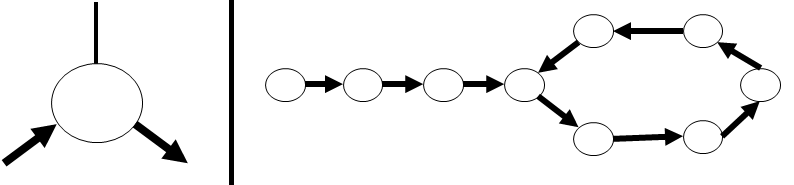
\includegraphics[width=0.5\textheight]{img/sinklessProof}
	\caption{As an orientation order consists of a directed path connected to a cycle (where each vertex has out-degree $> 1$), each order encountered by a vertex has an order to orient one of its an edges outwards from it, so such an edge associated with the highest id encountered is oriented outwards at the end of the algorithm.}
\end{figure}

\begin{theorem}
$SinklessLocal$ is a procedure that outputs a sinkless orientation and terminates after $O(\log{n})$ rounds.
\end{theorem}

%%%%%%%%%%%%%%%%%%%%%%%%%%%%%%%%%%%%%%%%%%%%
\section{Randomized Sinkless algorithm using Algorithmic local Lemma}
\label{sec:rand_lovasz}
This section aims to reduce the sinkless orientation problem for $d$ regular graph to the Distributed Lovaz Algorithmic local Lemma (LLL) with variable dependency $d$ (To be defined later). The first result gives a reduction from LLL to any $d$ using an assumption of $d$-edge coloring, which is sufficient for the original lower bound purposes, and the second result shows how to lift the need of $d$-edge coloring using maximal matching, and extending the results to many related problems, such as sinkless sourceless orientation.

\subsection{Distributed Algorithms for the Lovasz Local Lemma }
The setting of the Symmetric Algorithmic Lovasz Local Lemma by Moser and Tardos \cite{MoserT10} is the following: 
\begin{problem}[Moser and Tardos]
Let $P$ be a finite set of mutually independent random variables in a probability space. Let $\mathcal{A}$ be an set of events, $p \in [0,1]$ such that  for any event $A \in \mathcal{A}$, $Pr(A) \leq p$ , and each event in $\mathcal{A}$ share variables with at most $d$ other events. Given that $ep(d+1) < 1$, Find an assignment for all variables such that no event in $\mathcal{A}$ occurs.
\end{problem}

the dependency graph $G_{\mathcal{A}}$, is defined as a graph where each $A \in \mathcal{A}$ is a vertex, and two vertices have an edge if they share common variables (are Dependant). In the distributed model we assume that our communication graph is the dependency graph, and our goal is for each vertex to output a value of its variables such that the problem no $A \in \mathcal{A}$ occurs.

In $\cite{KMPHH14}$, two distributed LLL algorithms were developed for the LOCAL model, with slightly different dependence assumptions. Given  $ep(d+1) < 1$, there is an algorithm  for solving a LLL instance in running in $O(log^2(d) \cdot \log{n})$ rounds, and given $epd^2 < 1$ it can be done in $O(\log{n})$ rounds. 

\begin{definition}
Given a d-regular graph $G=(V,E)$, define a random variable for each edge to be its direction, and for each $v \in V$ define a bad event $A_v=$"$v$ is a sink" ($out\text{-}deg(v) = 0$). Let $G_{Sink}$ be the dependency graph of these bad events and probability space. 
\end{definition} 
\begin{lemma}
	\label{lem:rand_sink_dep_graph}
The following observations hold for $G_{Sink}$:
\begin{compactenum}
\item $A_v$  shares variables with  $A_u$ if and only if $(u,v) \in E$.
\item The dependency graph $G_{Sink}$ is isomorphic to $G$, and  $\phi(v) =A_v$ is an isomorphism function.
\item $Pr(A_v) = \frac{1}{2^d}$	
\end{compactenum}
\end{lemma}
\begin{proof}
For (1), since the independent variables are the edge directions, if $u,v$ are not neighbors, then "$u$ is a sink" and "$v$ is a sink" do not share a common variable. In the other direction if $u,v$ are neighbors and $u$ is a sink, then the edge between $u$ and $v$ must be directed $(v,u)$, meaning $v$ isn't a sink, thus $A_v$ and $A_u$ are dependent. Note that (2) follows immediately from the first claim and the definition of the dependency graph. 

Claim (3) holds since $G$ is a d-regular graph, so the probability of a bad event $A_v$ is $\frac{1}{2^d}$, as the edge directions are chosen i.i.d uniformly.
\end{proof}


\subsection{$O(\log{n})$ Algorithm on d-regular graphs with $d > 3$}
This subsection gives the description of the algorithm for $d > 3$. This follows directly by applying the LLL algorithm.

\begin{lemma}
Given a 4-regular graph, a sinkless orientation can be found in $O(\log{n})$ rounds using the distributed algorithmic local lemma.
\end{lemma}
\begin{proof}
For an i.i.d random choice of edge directions,  it holds that for any $A_v$,  $ P(A_v) = \frac{1}{16}$, meaning $ep(d+1) = \frac{e \cdot 5}{16} < 1$, therefore by the distributed algorithmic local lemma it can be solved in $O(\log{n})$ rounds.  
\end{proof}

\begin{corollary}
Given a d-regular graph, $d > 3$, a sinkless orientation can be found in $O(\log{n})$ rounds using the distributed algorithmic local lemma.
\end{corollary}
\begin{proof}
	For $4 \leq d \leq 8$ the algorithm in $\cite{KMPHH14}$ terminates after $O(log^2(d) \cdot \log{n}) = O(\log{n})$ rounds w.h.p, and gives direction assignments to each edge. For $d > 8$ the stronger $epd^2 < 1$ holds so using the second LLL algorithm in$\cite{KMPHH14}$, an LLL can be obtained in $O(\log{n})$ rounds.
\end{proof}

\subsection{$O(\log{n})$ Algorithm on 3-regular graphs}
Unfortunately, for the 3-regular case, the Local Lemma is not directly applicable since $ep(d+1) > 1$. We show a reduction to the 4-regular case. 

The key observation is that two 3-degree adjacent vertices act together like a single 4-degree vertex: if we contract the two adjacent vertices into one by their common edge, the new vertex has 4 edges, and if the graph was directed the new vertex isn't a sink if and only if in the original graph we can redirect the inner edge such that they are both not a sink.

\begin{figure}[h]
\centering
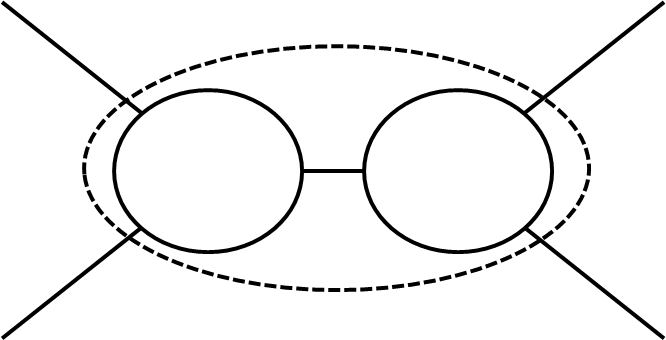
\includegraphics[width=0.5\textwidth]{img/RandomizedReductionContraction}
\caption{Contracted 3-degree vertices act like a 4-degree vertex}
\label{figure:RandomizedReductionContraction}

\end{figure}



\subsubsection{Reduction for 3-edge-colored graph}
For the purpose of showing lower bounds on the local lemma in the LOCAL model, it is sufficient to show it for 3-edge-colored 3-regular graphs.  Using the observation above, we note that each of the three edge colors form a perfect matching.


\begin{algorithm}[H]\label{Graph reduction algorithm_colored}\small
	\caption{\small Graph reduction algorithm($DependancyGraph$)}
	\begin{itemize}
		\item Take $M$ to be the perfect matching which is the set of edges of color $1$.
		\item Contract vertices sharing edges $(u,v) \in M$. (contraction may create double edges)
		\item Denote $G'$ as the multi-graph  created by this process
	\end{itemize}
\end{algorithm}

We note that each vertex $v$ in $G'$ has degree exactly $d(v)=4$, and that Any distributed algorithm on $G'$ can be simulated by $G$ with constant overhead, by having a contracted node in $G'$ be simulated by the two nodes in $G$ that form it.  

\begin{lemma}
	Given a sinkless orientation on $G'$, a sinkless orientation can be found on the network $G$ in constant time.
\end{lemma}
\begin{proof}
	Consider a partial orientation on $G$ induced by  the uncontracted edges in $G$ (which are the edges in $G'$), and giving them the same orientation. If $G'$ is sinklessly oriented, then each matched pair has an edge leaving one of its vertices. Direct each of the contracted edges so that both matched vertices touching each edge are satisfied. This is possible since if a contracted vertex $w_{uv}$ isn't a sink in $G'$, then it has an outgoing edge, meaning that in $G$ either $u$ or $v$ have an outgoing edge, and therefore isn't a sink. Assume w.l.o.g that $v$ isn't a sink, then directing the edge $\{v,u\}$ towards $u$ makes it so both $v$ and $u$ are not sinks
\end{proof}

All that remains is to obtain a sinkless orientation for multi-graphs of degree $4$. This can be obtained using the distributed LLL similar to the $4$-regular case. By choosing the edge direction at random, the probability that a vertex is a sink is exactly $\frac{1}{2^4}$, on the other hand, each vertex has of at most $4$ distinct neighbors, therefore it has degree at most $4$ in the dependency graph. since $ep(d+1) = e\frac{5}{16} < 1$, we obtain a sinkless orientation via the use of the distributed local lemma, which concludes the reduction.


\subsubsection{Algorithm for general 3-regular graphs}

In the previous case, we used a perfect matching to reduce to the 4-regular case. a perfect matching is sufficient, but don't necessarily exist, or are hard to obtain in general $3$-regular graphs. In this subsection we show that a maximal matching is sufficient for the reduction. This is not needed for the lower bound on the Lovasz Local Lemma, but can be used as a tool to solve variants of the sinkless orientation, such as sinkless sourceless orientation. To find a maximal matching $M$, and contract matched vertices into a new 4-degree vertex (figure \ref{figure:RandomizedReductionContraction}). After that, the graph is almost a 4-regular graph, up to the unmatched isolated vertices. These will be forced by the reduction to act as an edge between two neighboring 4-degree vertices (figure \ref{figure:RandIsoVert}). 

\begin{figure}[h]
	\centering
	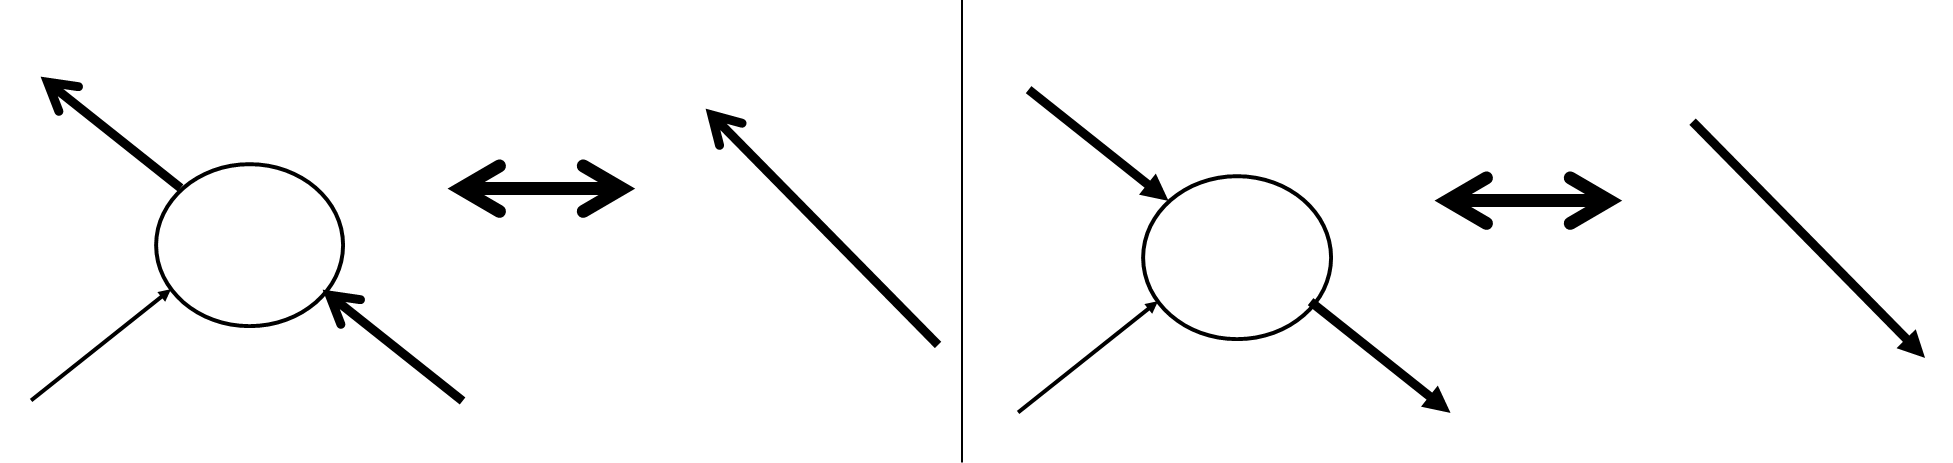
\includegraphics[width=1.0\textwidth]{img/RandomizedReductionIsolatedVertex}
	\caption{After fixing one of their edges inward, we can make isolated unmatched vertices acts as an edge between two matched neighboring vertices}
	\label{figure:RandIsoVert}
\end{figure}
\begin{algorithm}[H]\label{Graph reduction algorithm}\small
\caption{\small Graph reduction algorithm($DependancyGraph$,$M$)}
Denote the multi-graph created by this process $G'$:
\begin{itemize}
\item Contract vertices sharing edges $(u,v) \in M$. (contraction may create double edges)
\item For each isolated unmatched vertex $u$, replace two arbitrary edges $(u,v_1),(u,v_2)$ with an edge $(v_1,v_2)$, and remove the vertex and third edge
\end{itemize}
\end{algorithm}



\begin{lemma}
Given an orientation on $G'$ such that each $u \in \{v|d(v)=4\}$ is not a sink, a sinkless orientation can be found on the network $G$ in constant time.
\end{lemma}
\begin{proof}
\label{LLLThreeRegComplexLemma}
For each edge in $G'$ created by two edges of an isolated vertex $u$ in $G$, direct them both as directed by $G'$ as shown in figure \ref{figure:RandIsoVert}. Direct the third edge of an isolated vertex into the isolated vertex. The remaining non-matching edge in $G$ exist in $G'$ and direct them the way it is directed in $G'$. For isolated vertices, we note that no matter how we orient an edge in $G'$, it has an outgoing edge. Since it is a sinkless orientation in $G'$, then each matched pair has an edge leaving one of its vertices. Direct the edges in the matching $M$ so that both matched vertices are satisfied. This is possible since if a contracted vertex $w_{uv}$ isn't a sink in $G'$, then in $G$ either $u$ or $v$ isn't a sink.
\end{proof}

\begin{lemma}
Directing $G'$ to an orientation such that all 4-degree vertices are not a sink can be reduced to solving an LLL instance of the same size.
\end{lemma}
\begin{proof}
This is similar to the 4-regular case. Choose a random orientation for all edges in $G'$. In this case only 4-degree vertices sinks are considered bad events, and we note that the dependency graph has dependency $4$, and each two vertices in the dependency graph are at most of distance $2$ in the communication graph. Bad events as before have $Pr(A_v) \leq \frac{1}{16}$ as each of their edges are chosen uniformly and independently.  Since $ep(d+1) = e\cdot \frac{1}{16}\cdot 5 < 1$, it follows that the LLL algorithm converges after $O(log^2(d) \cdot \log{n}) = O(\log{n})$ rounds, meaning we get an orientation such that any $u \in \{v|d(v)=4\}$ isn't a sink. From Lemma \ref{LLLThreeRegComplexLemma} we can obtain a sinkless orientation on $G$ in constant time.
\end{proof}


\begin{algorithm}\label{ThreeRegularReduction}\small
\caption{\small ThreeRegularReduction($DependancyGraph$)}
\begin{itemize}
\item Obtain a MIS $M$ of $G$.
\item Calculate $G'$ using $M$
\item Run an LLL algorithm on the graph $G'$
\item Translate the directions into $G$ in the following manner:
\begin{itemize}
\item If $e \in G'$ is an edge in both $G$ and $G'$ direct it in the same manner as $G'$.
\item If $e \in G'$ was created by two edges of an isolated vertex, direct them the same way as the edge in $G'$ as shown in figure \ref{figure:RandIsoVert}.
\item If $e=(u,v)$ ia an edge in $M$, then direct it so that both $u$ and $v$ aren't sinks
\end{itemize}
\end{itemize}
\end{algorithm}

\begin{theorem}
 A 3-regular graph sinkless orientation instance can be reduced to a Distributed Lovasz Local Lemma instance in $O(log^*n)$ rounds.
\end{theorem}
\begin{proof}
Obtaining an MIS takes $O(\log^* n)$ rounds on bounded degree graphs, reduction to $G'$ takes $O(1)$ rounds, And by using the LLL algorithm on $G'$ the instance can be solved.
\end{proof}
\begin{corollary}
Sinkless orientation on 3-regular graphs can be solved in $O(\log n)$ rounds.
\end{corollary}

\subsection{Conclusion}
We've studied the sinkless orientation problem, shown a deterministic algorithm, and shown a reduction to the Lovasz Local Lemma in regular graphs, overcoming a difficulty in the case $d=3$, where the LLL criteria is too weak for it. We note that using the distributed algorithmic Lovasz Local Lemma we can solve similar problems to the sinkless orientation, such as sinkless sourceless orientations, even if at first they don't seem to meet the criteria of the LLL using the tools in the final subsection. This is done iteratively by constructing a new multi-graph by gaining a maximal matching, amplifying the success probability of each bad event, until the LLL criteria is met.

\section{An $O(\log{n})$ Deterministic Algorithm For Sinkless Orientation in the CONGEST model}
 A natural question regarding Sinkless orientation is if it can be done efficiently while restricting the edge bandwidth in each round to be $O(\log{n})$ (i.e the CONGEST model). For a randomized protocol, the LLL algorithm of \cite{KMPHH14} gives us an immediate positive answer. This is due to the fact that their algorithm consists of finding a maximal independent set of bad event vertices in the dependency graph and re-sampling them, but the bad events defined in section \ref{sec:rand_lovasz} clearly form an independent set, as if $v$ is a sink, then all of its neighbors in $G$ must not be sinks, as they have an outgoing edge to $v$, and so by lemma \ref{lem:rand_sink_dep_graph} part (2) the claim follows. For a deterministic algorithm, naively implementing the algorithm in section \ref{AlgSection} would not work, as each vertex learns its $\log{n}$ neighborhood, and therefore has a very high message length. in the following section we give an efficient algorithm for sinkless orientation in a restricted bandwidth model to the deterministic case as well.

In this algorithm, having vertices attempt to orient a path connected to a cycle plays a key role as well, but we can't have each vertex learning such a path and cycle, as it might be too expensive to do in parallel. 

\begin{definition}
	$v$ is a dominating vertex if it has the maximum id in its $2\log{n}$ neighborhood
\end{definition}
Each dominating vertex can safely perform a BFS on its $\log{n}$ neighborhood without interference from other dominating vertices. It is not clear how such a vertex learns the path and cycle in a restricted bandwidth setting. For this we define cycle witnesses
\begin{definition}
	Denote a vertex $u$ a witness cycle from a vertex $v$ with regards to a BFS protocol originating from $v$ if it has received at least two incoming messages during the BFS.
\end{definition}
We note that these messages must be received in two different edges.The key idea of the algorithm is as follows: each dominating vertex $v$ orients a path and a cycle. It does so by performing a BFS on its $\log{n}$ neighborhood, finding a cycle witness $u$. By definition a cycle witness has two edges in which it has received a BFS message. By considering two tokens - a red token and a blue token, each starting at $u$. $u$ sends one token through each such edge, and then the token backwards traversal through the BFS up to the root $v$. We note that the edges on which a token was traveresed form a path connected to a cycle (See figure). Oriented correctly, this yields a directed path starting from $v$, connected to an oriented cycle that contains $u$. The process above satisfies the dominating vertices, and the part of their $\log{n}$ neighborhood participating in the path and cycle defined above (denoted active nodes in the algorithm). The rest of the vertices are not satisfied by this process, but as will be shown later, is sufficient if each non-active (passive) vertex picks the edge from its edges that is closest to the largest id in its $2\log{n}$ neighborhood ($passiveParent$) and orient it outwards.

\begin{figure}[h]
	\centering
	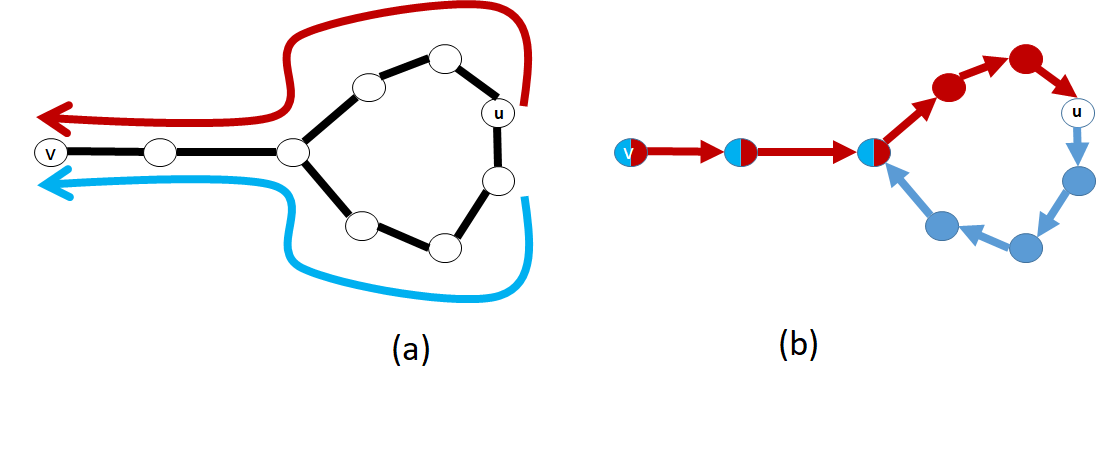
\includegraphics[width=0.8\textwidth]{img/CongestFigure.png}
	\caption{\\(a) The path of the tokens from the chosen witness $w$ to its dominating vertex $v$ \\(b)The orientation each edge receives in this process.If it seen only blue - towards parent,if it seen red - towards child}
\end{figure}



\begin{algorithm}[H]\label{alg:sinkless_congest}\small
	\caption{\small SinklessCongest($G$)}
	\begin{itemize}
		\item Using a priority BFS for $2\log{n}$ rounds from all vertices, each vertex checks if it is a dominating vertex, and if not it saves two pointers - $passiveRoot,passiveParent$ as the maximum id encountered and the edge in which it entered the earliest (breaking ties by ids of parents).
		\item Each dominating vertex starts a BFS for $\log(n)$ rounds. Note that as two dominating vertices have a distance of at least $2\log{n}$, the two BFS originating from them are disjoint
		\item All cycle witnesses of a vertex $v$ from the BFS send their id through their parent vertex in the BFS up to their root by priority BFS for $\log(n)$ steps. 
		\item If a dominating vertex $v$ receives a cycle witness, it chooses the cycle witness with the largest id and sends it to its $\log{n}$ neighborhood
		\item The chosen witness of $v$ chooses two incoming edges of the BFS, sends a red token through one, and a blue token through the second. These tokens traverse back through the parent edges until reaching back to $v$. 
		\item Through each edge that the red token traversed, direct the parent edge towards the child. If the blue token passes to the parent edge, and the red token did not, direct it towards the parent. If a vertex encounters any token in this phase, it marks itself as active, otherwise it marks itself passive
		\item Each passive vertex directs its $passiveParent$ edge outwards  
		\item Direct any undirected edge into the larger id 
	\end{itemize}
\end{algorithm}

\begin{lemma}
	Each dominating vertex receives a cycle witness during the algorithm.
\end{lemma}
\begin{proof}
	As two dominating vertices have distance at least $2\log{n}$, the BFS is uninterrupted by other dominating vertices.By Lemma \ref{lem:near_cycle}, each vertex has a cycle of length $\log{n}$ in its $\log{n}$ neighborhood. Therefore in a BFS of length $\log{n}$, at least one vertex from that cycle receives two messages.
\end{proof}

\begin{lemma}
	\label{lem:active_good}
	Edges oriented by active nodes of a dominating vertex $v$ before the end of the algorithm form a directed path connected to a directed cycle, where each edge is between two active vertices.
\end{lemma}
\begin{proof}
	Let $u$ be the chosen witness of $v$. All such edges are oriented by the red and blue token traversal. As the red and blue tokens originate together from $u$, and they move at the first step into two different vertices, and both reach $v$, there must be a vertex $w$ in which they both "re-meet" (in the sense that they both go through $w$). Furthermore, as they both traverse on parents of the BFS, once they "re-meet", the path traversed from $w$ to $v$ is traversed from both. The union of the two (disjoint) paths traversed up to $w$ is $u$ by both tokens form a cycle, and the path from $w$ to $v$ forms a path. The way the algorithm orients them forms a directed path, connected to a directed cycle. Clearly all nodes with edges oriented this way in the algorithm have a token traversing through them, therefore all edges are between two active vertices.  
\end{proof}
\begin{lemma}
	Edges orientations  of the algorithm are well defined.
\end{lemma}
\begin{proof}
	Consider the edges oriented before the last step. By Lemma \ref{lem:active_good}, all edges oriented by active nodes of a dominating vertex $v$ form a path connected to a cycle and are well defined. A passive vertex only orients the edge $passiveParent$. If its $passiveParent$ is between two passive nodes, the edge orientation is well defined unless the two vertices have the same edge pointer of $passiveParent$.  They have to be different, as if the $id$ of $passiveRoot$ is the same at both vertices, then the earliest entry time of the message to their $passiveParent$ edge differs by one, by definition of BFS, indicating that $passiveParent$ is not the same edge. In the case that $passiveRoot$ is different in these two vertices, which clearly indicates that $passiveParent$ is different. If the edge is between a passive and active node it is well defined as by Lemma \ref{lem:active_good} all edges oriented by active nodes are between two active nodes. Clearly all remaining unoriented edges in the last step are oriented in a consistent manner.
\end{proof}
\begin{corollary}
	\label{lem:congest_is_sinkless}
	The oriented edges of $G$ form a sinkless orientation.
\end{corollary}
\begin{proof}
	As each passive vertex has an outgoing edge to its $passiveParent$, and each active vertex has an outgoing edge as it participates in a directed path that connects into a directed cycle, all vertices have an outgoing edge.
\end{proof}

\begin{theorem}
	SinklessCongest terminates after $O(\log{n})$ rounds and  the orientation obtained is a sinkless orientation.  
\end{theorem}
\begin{proof}
	The round complexity is clearly $O(\log{n})$, as the time complexity of each step is bounded by at most $2\log{n}$ rounds, and by Corollary \ref{lem:congest_is_sinkless} the orientation obtained is a sinkless orientation.   
\end{proof}
%% *** Include chapter files here. ***

%% This adds a line for the Bibliography in the Table of Contents.
\addcontentsline{toc}{chapter}{Bibliography}
%% *** Set the bibliography style. ***
%% (change according to your preference/requirements)
\bibliographystyle{alpha}
%% *** Set the bibliography file. ***
%% ("thesis.bib" by default; change as needed)
\bibliography{refs}

%% This adds the hebrew abstract and back cover to the thesis.
 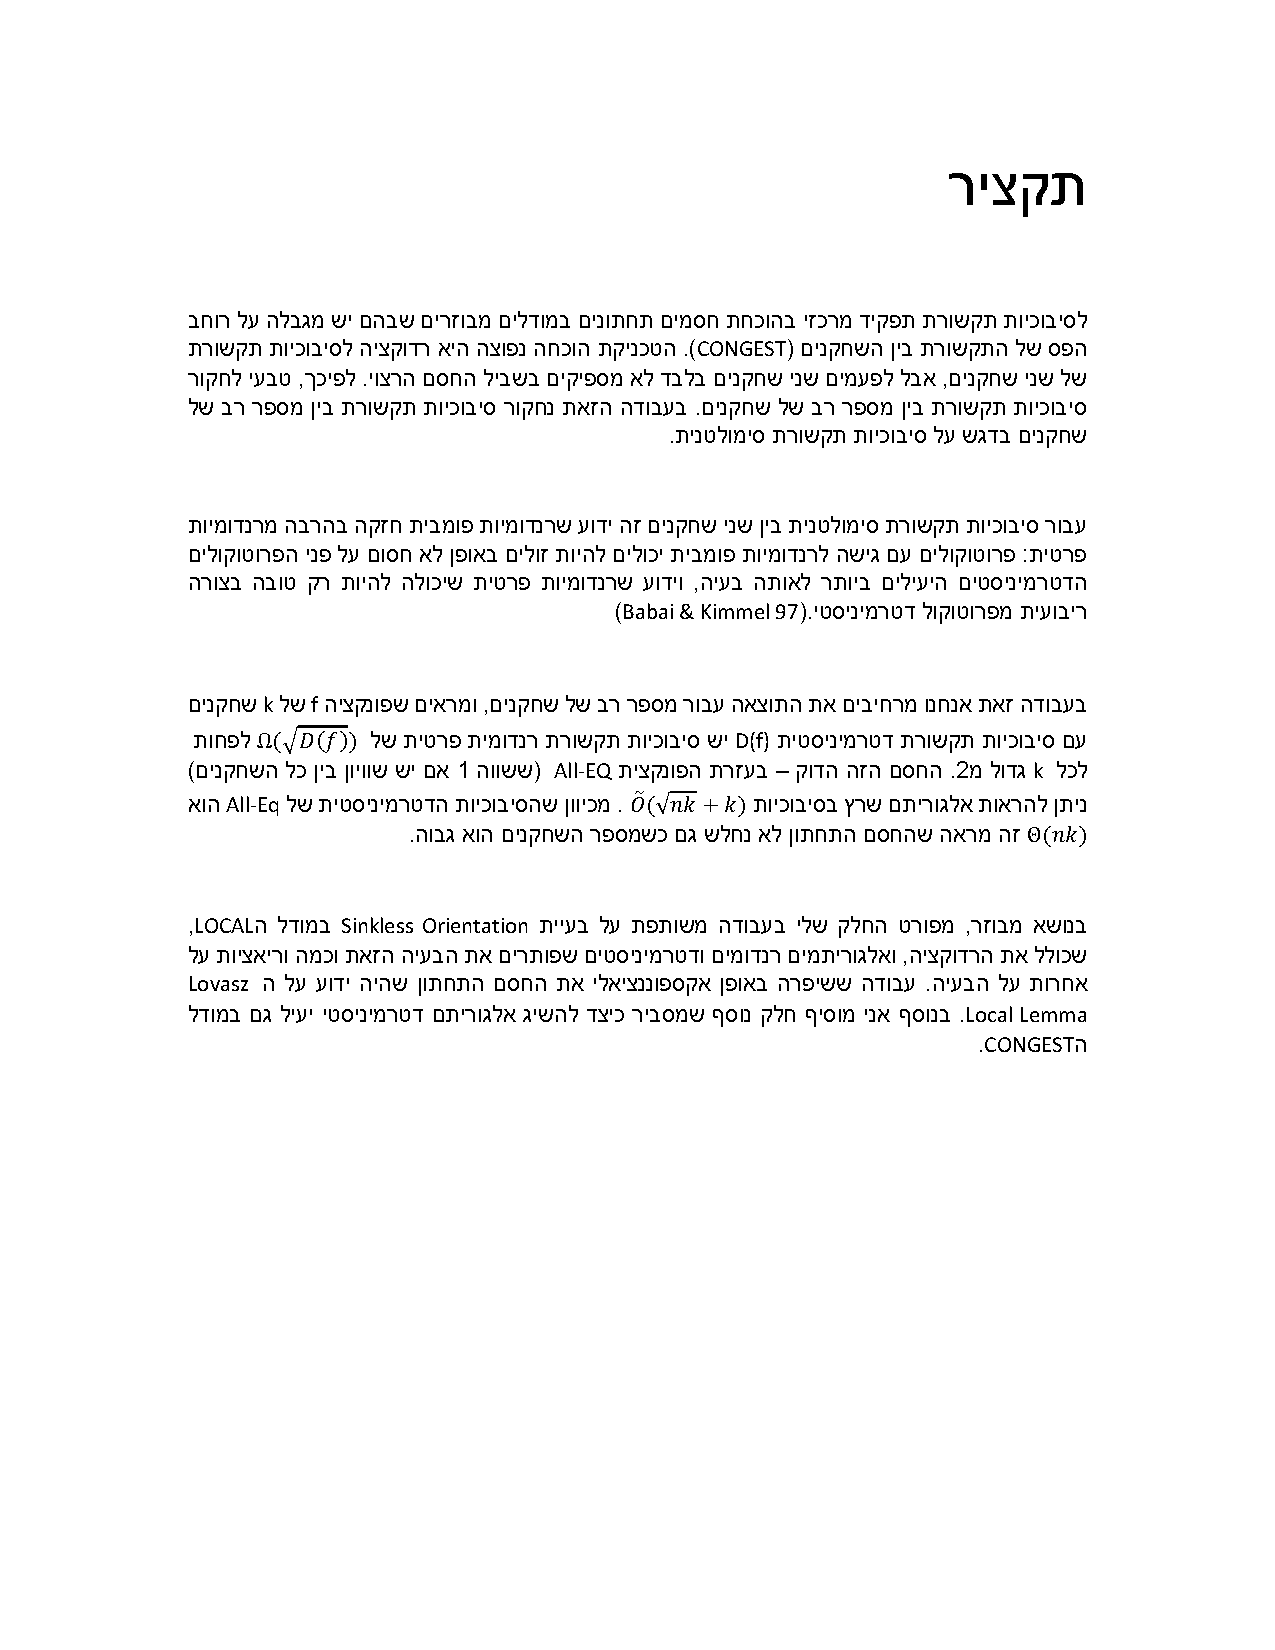
\includepdf[pages=-]{hebrew-abstract.pdf}

%% *** NOTE ***
%% If you don't use bibliography files, comment out the previous line
%% and use \begin{thebibliography}...\end{thebibliography}.  (In that
%% case, you should probably put the bibliography in a separate file and
%% `\include' or `\input' it here).

\end{document}